\chapter{Descrição do sistema}
\label{c.descricao-do-sistema}

O sistema como um todo segue uma arquitetura cliente-servidor, onde o usuário interage com uma aplicação cliente que, por sua vez, se comunica com um servidor através da internet utilizando algum protocolo de rede. A aplicação cliente, nesse caso, é um aplicativo para dispositivos móveis, enquanto o servidor é uma aplicação monolítica, ou seja, um serviço único que é executado em um único processo. Foi considerado o desenvolvimento de vários microserviços, porém a arquiteture monolítica foi escolhida em virtude da sua simplicidade de desenvolvimento, facilidade de testes e de \emph{deploy}. 

A Figura~\ref{f.system} ilustra os componentes físicos do sistema. A AWS (\emph{Amazon Web Services}) ~\cite{aws} é um provedor de serviços em nuvem. Dentre os seus serviços oferecidos, foi utilizado o Amazon S3 (\emph{Simple Static Storage}) para armazenamento de objetos estáticos (imagens e vídeos) e o Amazon RDS (\emph{Relational Database Service}) para o provisionamento do banco de dados PostgreSQL~\cite{postgresql}. O Heroku~\cite{heroku} é outro provedor de serviços em nuvem que foi utilizado para a implantação do servidor em produção e o provisionamento do banco de dados Redis~\cite{redis}.

\begin{figure}[htbp]
	\caption{\small Componentes físicos do sistema.}
	\centering
	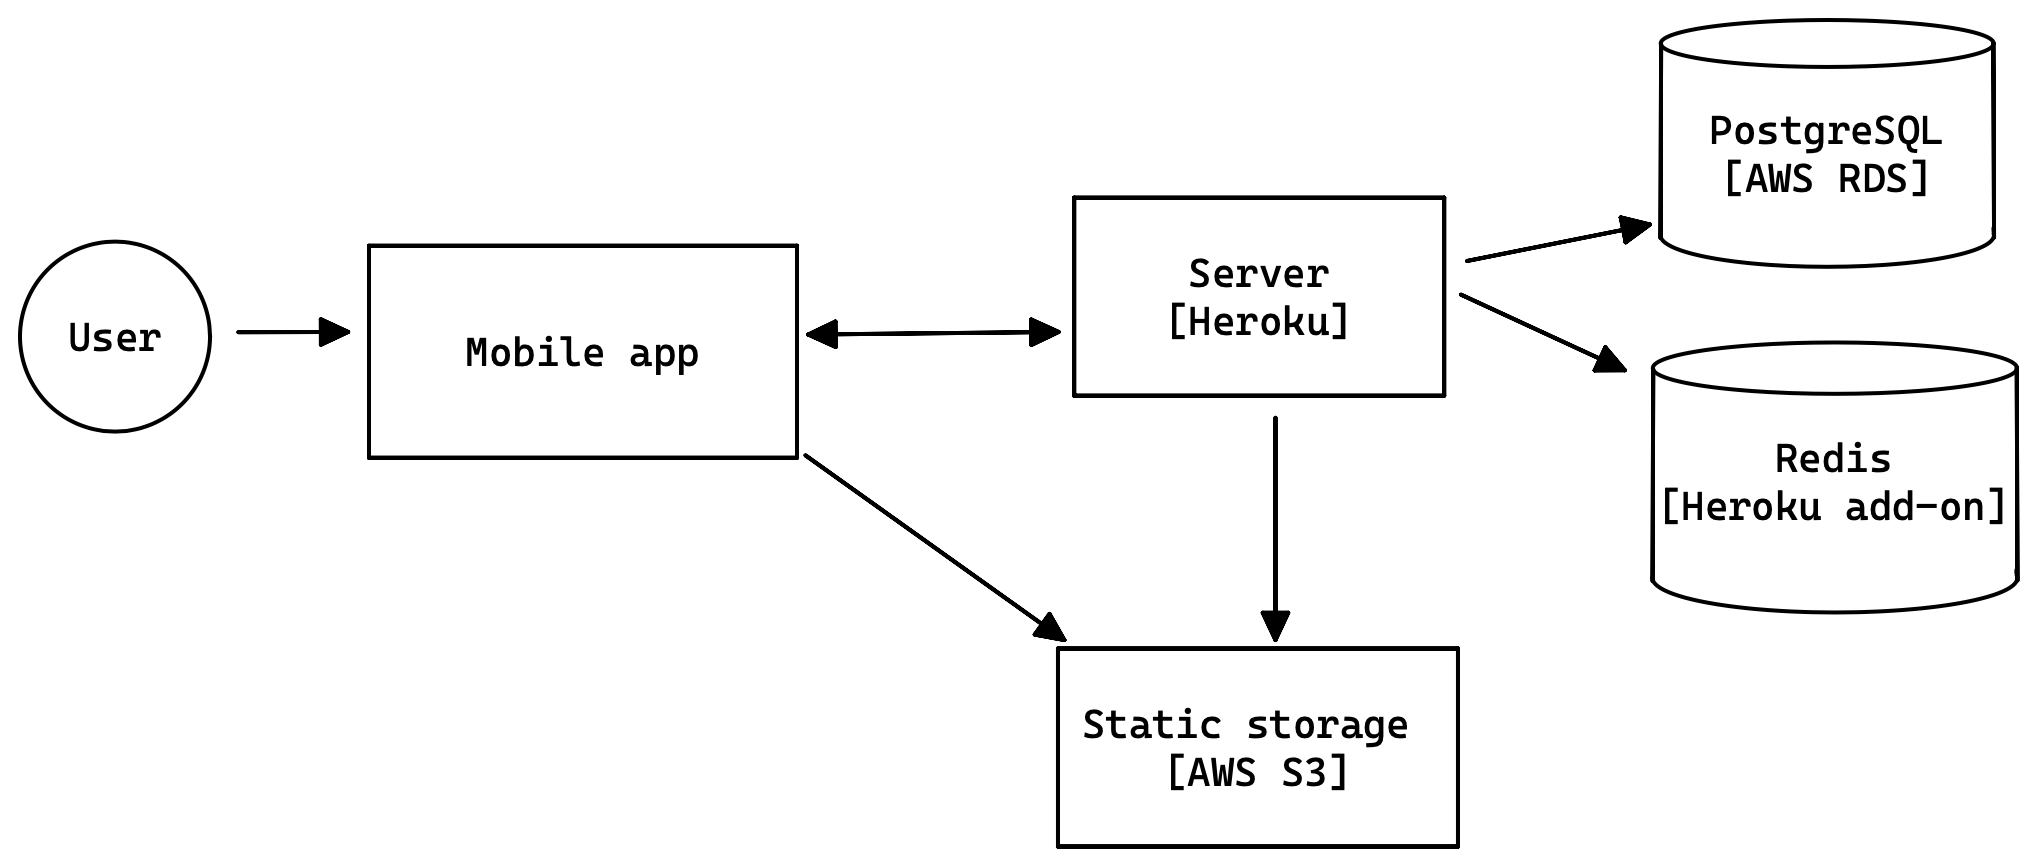
\includegraphics[width=\textwidth]{../diagrams/out/system.png}
	\label{f.system}
	\legend{\small Fonte: Elaborado pelo autor.}
\end{figure}

\FloatBarrier

\section{Servidor}

Os princípios do \emph{domain-driven design}, termo cunhado inicialmente por Eric Evans ~\cite{domain-driven-design}, e a ideias propostas por Uncle Bob em \emph{Clean Architecture} ~\cite{clean-architecture} tiveram grande contribuição para o projeto do servidor, tendo em vista que a \emph{separation of concerns} e a divisão da aplicação em camadas bem definidas com um rico modelo de domínio no centro permitem com que a complexidade do projeto cresça de forma manutenível ao longo do tempo.

A partir dos requisitos listados na Seção~\ref{s.requisitos}, se fez necessário identificar os diferentes subdomínios do sistema. Um módulo, também chamado de subdomínio, é um pedaço isolado de código. Como ilustrado pela Figura~\ref{f.system_server}, os seguintes módulos foram identificados:

\begin{itemize}
	\item \texttt{user}: responsável pelos usuários, gerenciamento de identidade, autenticação e autorização;
	\item \texttt{incident}: responsável por todas as operações relacionadas aos alertas;
	\item \texttt{notification}: responsável pelo envio de notificações aos dispositivos dos usuários;
	\item \texttt{shared}: módulo global para reuso de código entre diferentes módulos.
\end{itemize}

\begin{figure}[htbp]
	\caption{\small Visão geral do sistema.}
	\centering
	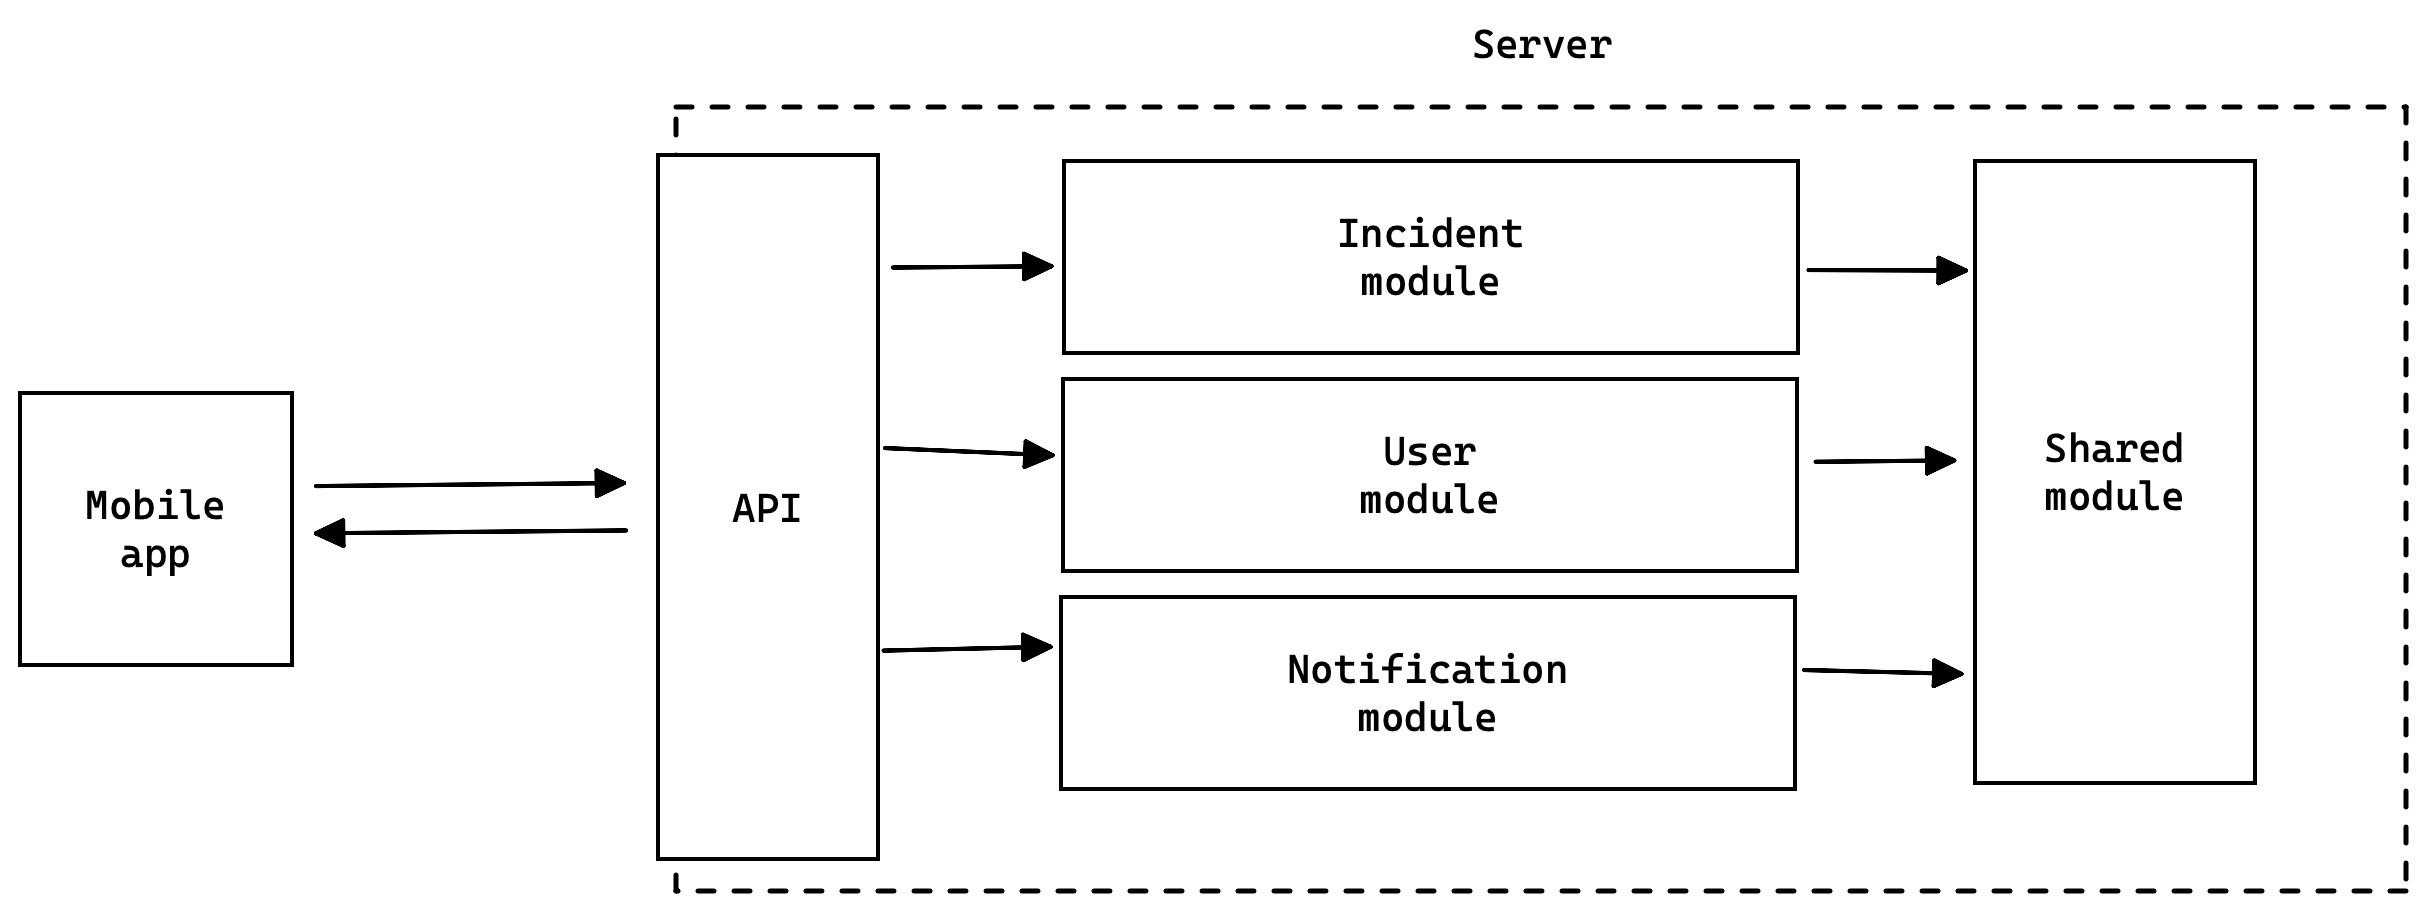
\includegraphics[width=\textwidth]{../diagrams/out/system_server.png}
	\label{f.system_server}
	\legend{\small Fonte: Elaborado pelo autor.}
\end{figure}

\FloatBarrier

\subsection{Principais tecnologias}

O servidor foi escrito utilizando Node.js~\cite{node}. O Node.js é um \emph{runtime} para Javascript~\cite{javascript} baseado no interpretador V8 do Google que é utilizado pelo navegador Google Chrome. O principal motivador de sua escolha foi pela sua característica de execução das requisições e eventos em \emph{single-thread}, ou seja, uma única \emph{thread} (chamada de \emph{event loop}) é responsável por executar o código Javascript e, portanto, recursos computacionais como memória RAM são melhor aproveitados. Outra característica que o difere de outras linguagens é que as suas operações de entrada e saída são assíncronas e não bloqueantes, o que torna aplicações orientadas à entrada e saída, como é o caso de servidores que processam inúmeras requisições recebidas pela rede em paralelo, bons casos de uso para o Node.js. 

O servidor possui dependência com algumas bibliotecas e frameworks do ecossitema Node.js. As principais são: Koa~\cite{koa}, um framework para contrução de servidores web; Prisma~\cite{prisma}, um ORM (\emph{Object-Relational Mapping}) para interação com bancos de dados; Jest~\cite{jest}, uma biblioteca para escrita de testes unitários; e Supertest~\cite{supertest}, uma bilioteca para a escrita de testes de integração.

Em relação aos bancos de dados com os quais o servidor interage, foram escolhidos o Redis~\cite{redis} e o PostgreSQL~\cite{postgresql}. 

O Redis é um banco de dados em memória de baixa latência que fornece diversas estruturas de dados otimizadas. A estrutura de chave-valor foi utilizada para o o armazenamentos dos \emph{access tokens} e \emph{refresh tokens} dos usuários, os quais são utilizados para o controle das sessões dos usuários. E a estrutura \texttt{GEOSET} foi utilizada para a implementação de consultas eficientes por latitude e longitude.

Já o PostgreSQL é um poderoso sistema de banco de dados objeto-relacional de código aberto com mais de 30 anos de desenvolvimento ativo que lhe rendeu uma forte reputação de confiabilidade, robustez de recursos e desempenho. Ele foi utilizado para a persistência dos dados dos usuários, dos alertas e das notificações.

\subsection{Camadas de cada módulo}

Cada um dos módulos respeita a divisão em camadas descrita pela Figura~\ref{f.system_server_each-module_layers}, onde camadas mais externas dependem das camadas mais internas e, consequentemente, camadas mais internas não conhecem camadas mais externas. 

\begin{figure}[htbp]
	\caption{\small Camadas de um módulo do servidor.}
	\centering
	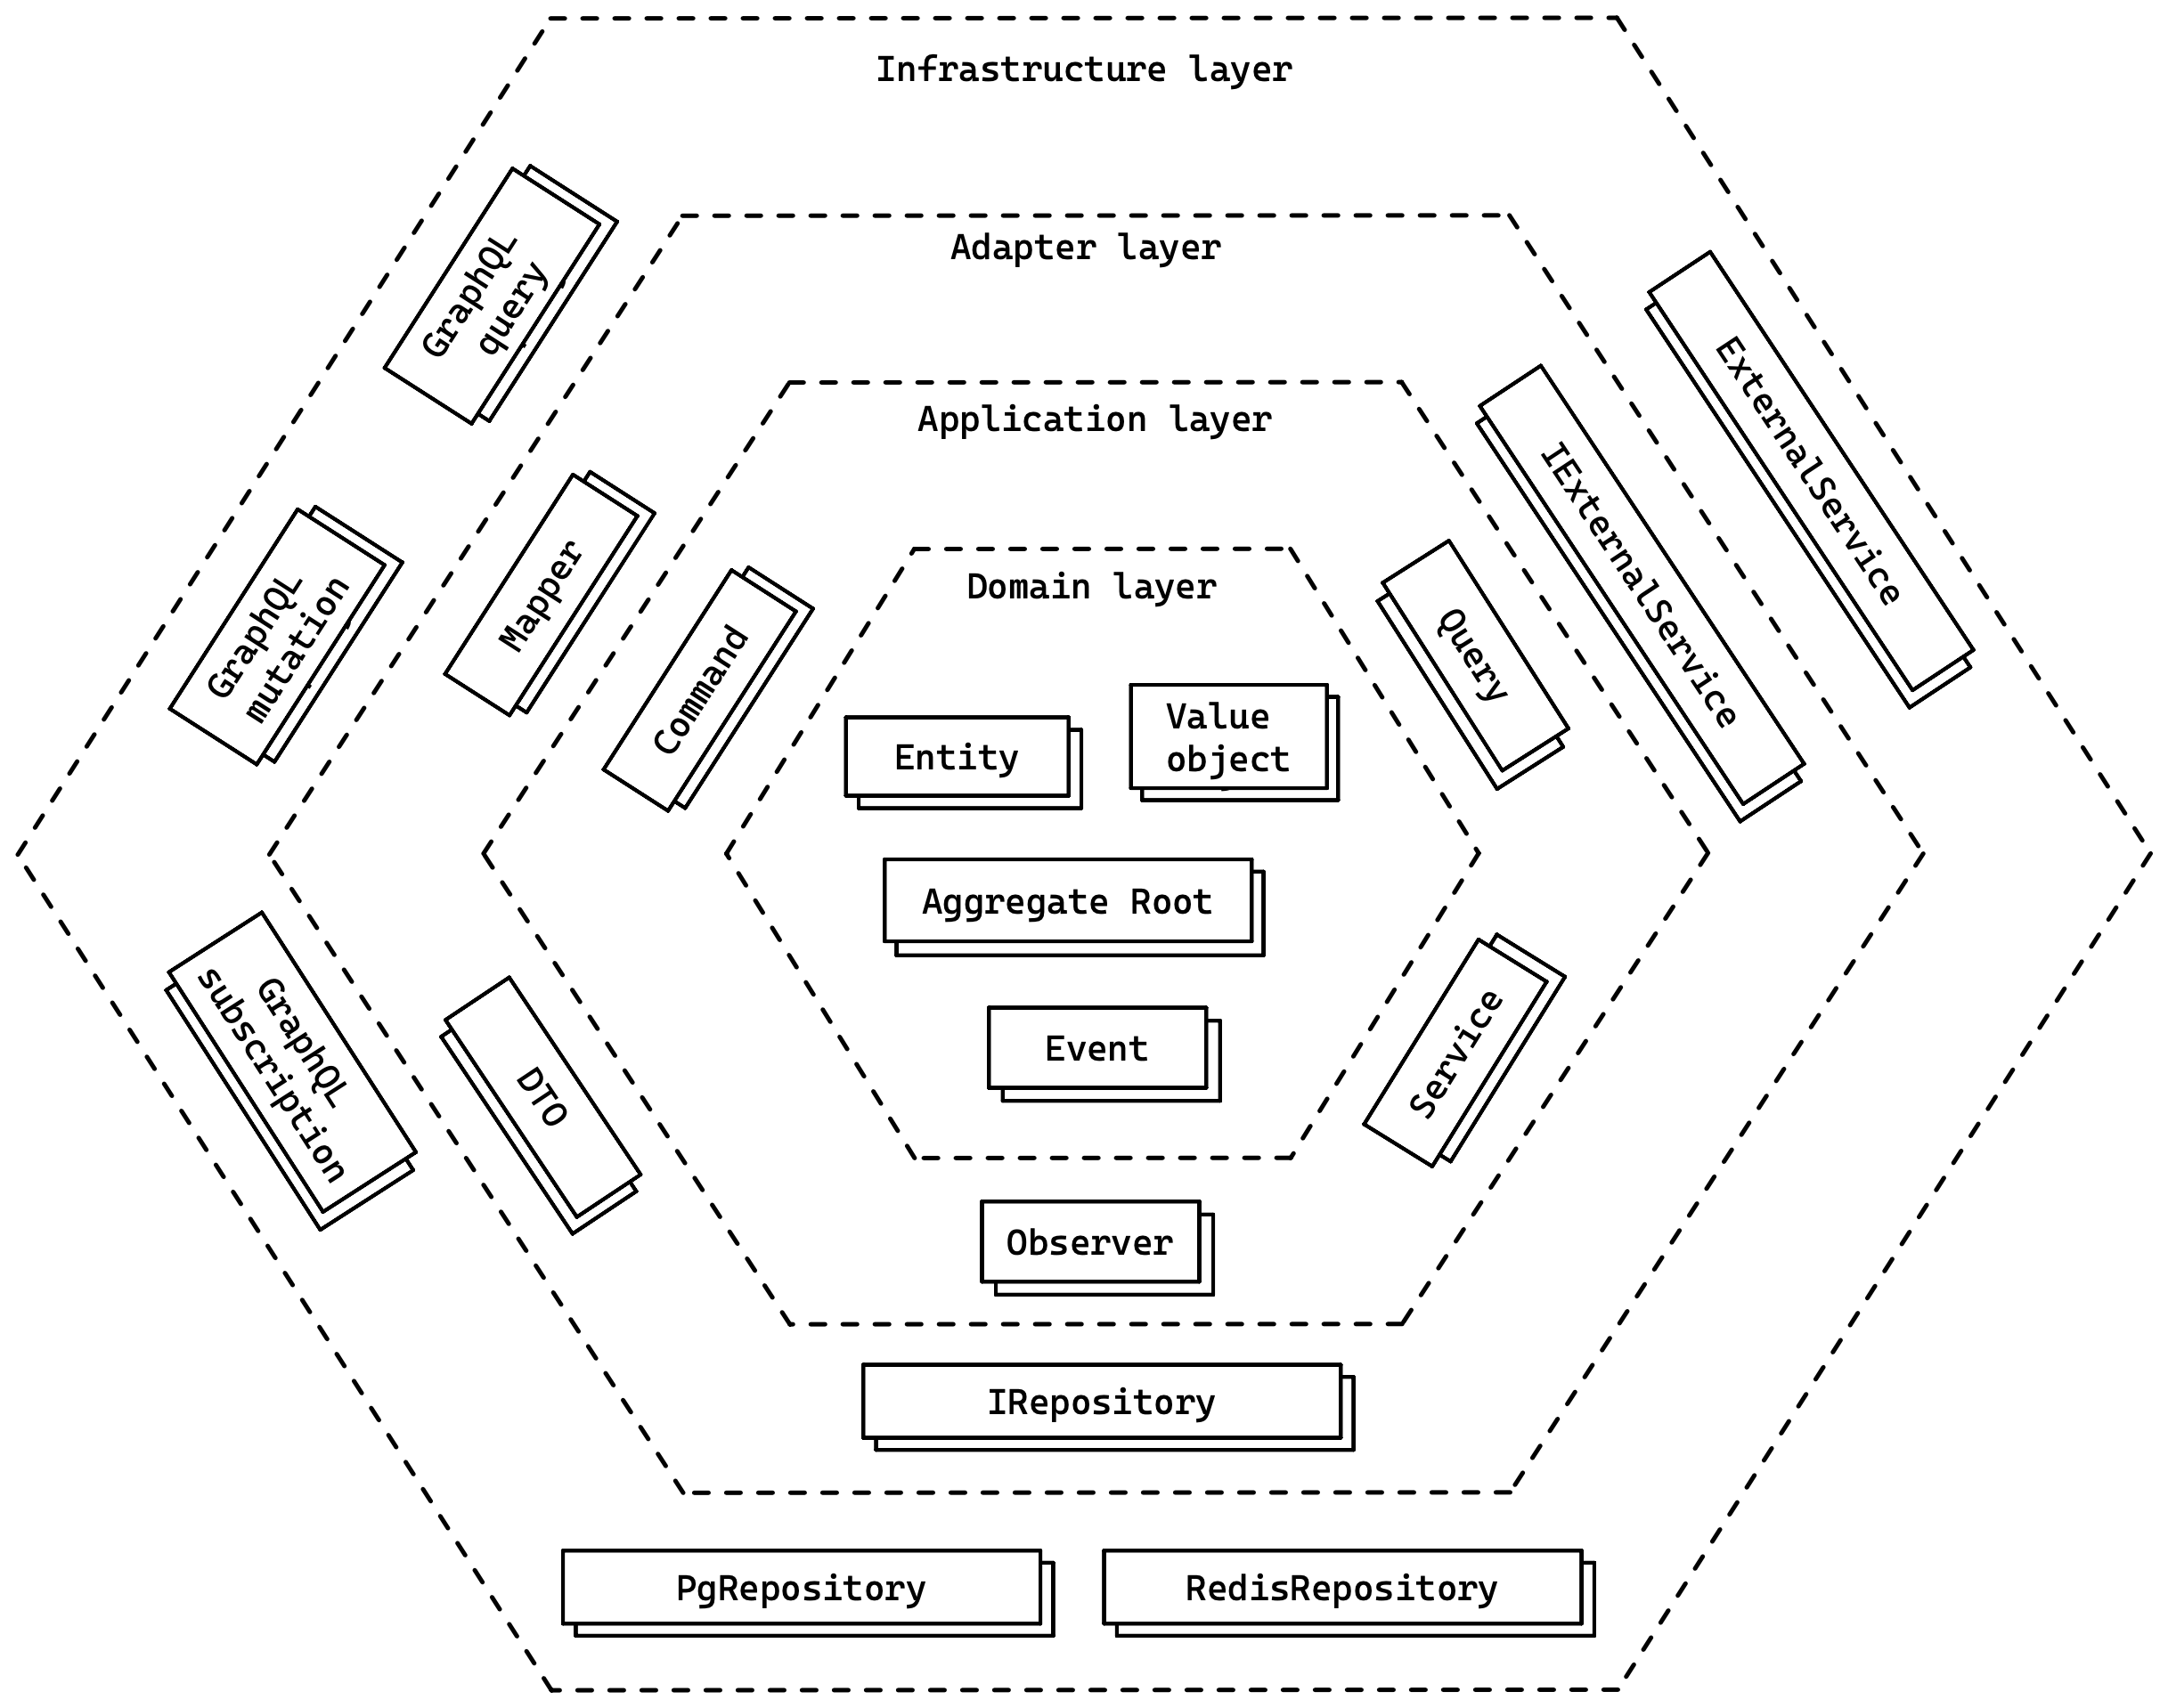
\includegraphics[width=\textwidth]{../diagrams/out/system_server_each-module_layers.png}
	\label{f.system_server_each-module_layers}
	\legend{\small Fonte: Elaborado pelo autor.}
\end{figure}

\FloatBarrier

De acordo com a ``arquitetura hexagonal'' de Alistair Cockburn ~\cite{hexagonal-architecture}, a região mais interna da arquitetura deve concentrar as camadas de aplicação e de domínio, e por fora dessas camadas devem estar os adaptadores (ou portas). 

A aplicação é escrita em cima das tecnologias específicas que existem no ``mundo exterior'', como bancos de dados, APIs (\emph{Application Programming Interface}) externas e serviços em nuvem. Com o uso dos adaptadores, ``o mundo exterior é conectado ao mundo interior'' e, portanto, tecnologias específicas podem ser envolvidos com segurança pela aplicação. Isso é chamado de inversão de dependência, e trás inúmeros benefícios, como: 

\begin{alineas}
	\item Atrasar a decisão sobre exatamente qual tipo de servidor web, banco de dados, serviços externos ou tecnologia de \emph{cache} será escolhido até que seja absolutamente necessário decidir. Facilitando, por exemplo, que se faça uma implementação inicial em memória do bancos de dados para agilizar o desenvolvimento;
	\item Prioriza a escrita de código que pode ser facilmente testado usando injeção de dependência, minimizando o uso de dependências concretas que poderiam tornar o código não testável; e
	\item Ajusta o foco às coisas específicas da aplicação e do domínio.
\end{alineas}

\subsubsection{Domínio}

A \texttt{domain layer} é a camada mais interna. É a camada que contém tudo aquilo que é importante para o negócio e que está menos propensa a mudar, configurando-se como a camada mais estável dentre todas e a qual todas as outras dependem.

Para encapsular regras de validação, existem os \texttt{value objecs}. Uma \texttt{entity} é um objeto que encorpa um pequeno conjunto de regras de negócio.

Um \texttt{aggregate root} é um tipo específico de \texttt{entity} que pode emitir \texttt{domain events} quando algo relevante para o negócio ocorre, e para isso, ele armazena como estado os eventos que ainda não foram emitidos pela camada de infraestrutura. Ele é implementado pela principal entidade de um \emph{cluster} de \texttt{entities} e \texttt{value objects} relacionados, os quais são tratados como uma única unidade de mudança.

A Figura~\ref{f.system_server_shared-module_domain} demonstra como essas classes abstratas são definidas no módulo \texttt{shared}, além da implementação da classe \texttt{DomainEvents}.

\begin{figure}[htbp]
	\caption{\small Diagrama de classes da camada de domínio do módulo compartilhado do servidor.}
	\centering
	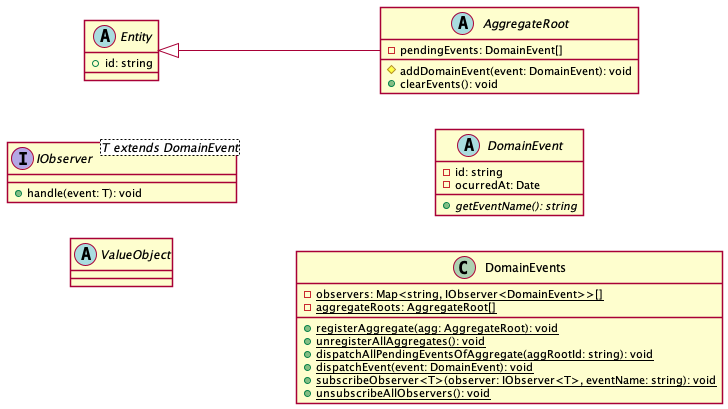
\includegraphics[width=\textwidth]{../diagrams/out/system_server_shared-module_domain.png}
	\label{f.system_server_shared-module_domain}
	\legend{\small Fonte: Elaborado pelo autor.}
\end{figure}

\FloatBarrier

A classe \texttt{DomainEvents} é um \emph{singleton}, ou seja, uma única instância global com tempo de vida vitalício em relação ao tempo de vida da aplicação. Ela é usada para encapsular o estado de quais \texttt{observers} estão interessados em ouvir pelos eventos emitidos por determinados \texttt{aggregate roots}. As instâncias dos \texttt{aggregate roots} inscritos contém \texttt{domain events} que serão dispachados para seus \texttt{observers} quando a camada de infraestrutura persistir as alterações feitas.

\subsubsection{Aplicação}

A \texttt{application layer} contém os casos de uso, ou seja, as principais funcionalidades da aplicação. Em relação ao ambiente externo as entradas são os \texttt{commands} e as \texttt{queries}, mas essa camada também implementa \texttt{application services} e \texttt{observers}, que são funções que serão executadas quando um determinado evento de domínio ocorre.

O \emph{Command-Query Separation (CQS)} é um padrão introduzido por Bertrand Meyer ~\cite{object-oriented-software-construction} que afirma que um método é ou um \texttt{command} que executa uma ação ou uma \texttt{query} que retorna dados ao chamador, mas nunca ambos. Dessa forma os fluxos de operações que mudam o sistema (e geram efeitos colaterais) são separados daqueles que apenas requisitam dados ao sistema, tornando o código mais simples de entender e manter.

\subsubsection{Adaptadores}

A \texttt{adapter layer} contém abstrações para que a \texttt{application layer} possa interagir com a \texttt{infrastructure layer} sem depender dela, habilitando o que é chamado de inversão de dependência. Interfaces de repositórios que acessam bancos de dados, interfaces ou classes abstratadas que chamam APIs externas e mapeadores de objetos entre diferentes camadas são exemplos do que pode estar nessa camada. Para que um objeto passe de uma camada à outra são utilizados DTOs (\emph{Data Transfer Object}). Toda entidade possui um modelo de domínio na \texttt{domain layer} e um modelo de persistência na \texttt{infrastructure layer}, por exemplo.

\subsubsection{Infraestrutura}

A \texttt{infrastructure layer} é a camada mais externa. Ela contém os detalhes da aplicação, os quais possuem maior chance de serem trocados por outras bibliotecas ou frameworks específicos ao decorrer do tempo. Isso inclui implementações concretas das abstrações definidas na \texttt{adapter layer} para que elas possam ser executadas em \emph{runtime}, como serviços externos, repositórios para acesso à bancos de dados. Além disso, também contém lógicas de apresentação, como \emph{HTTP (Hypertext Transfer Protocol) endpoints} e \emph{GraphQL operations}.

\subsection{Módulos}

Na sequência tem-se uma visão mais ampla de todos os módulos e como eles se inter-relacionam. Um módulo apenas deve se comunicar com outro via eventos de domínio, permitindo o desacoplamento entre eles.

A Figura~\ref{f.system_server_all-modules_domain-entities} ilustra como as entidades de cada módulo estão definidas. 

\begin{figure}[htbp]
	\caption{\small Diagrama de classes das entidades de domínio de cada módulo do servidor.}
	\centering
	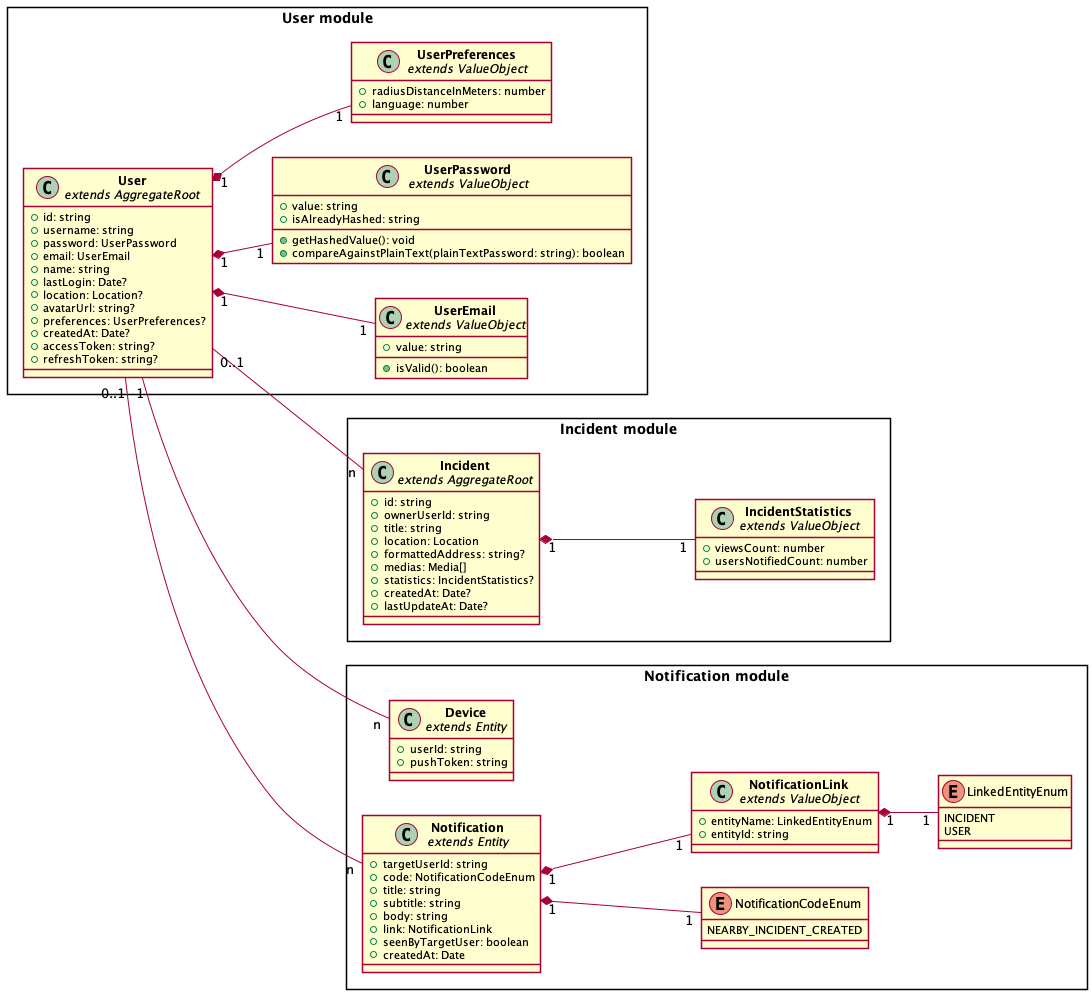
\includegraphics[width=\textwidth]{../diagrams/out/system_server_all-modules_domain-entities.png}
	\label{f.system_server_all-modules_domain-entities}
	\legend{\small Fonte: Elaborado pelo autor.}
\end{figure}

\FloatBarrier

A Figura~\ref{f.system_server_all_modules_commands-observers-events} ilustra as entradas e saídas de cada módulo.

\begin{figure}[htbp]
	\caption{\small Entradas e saídas de cada módulo do servidor.}
	\centering
	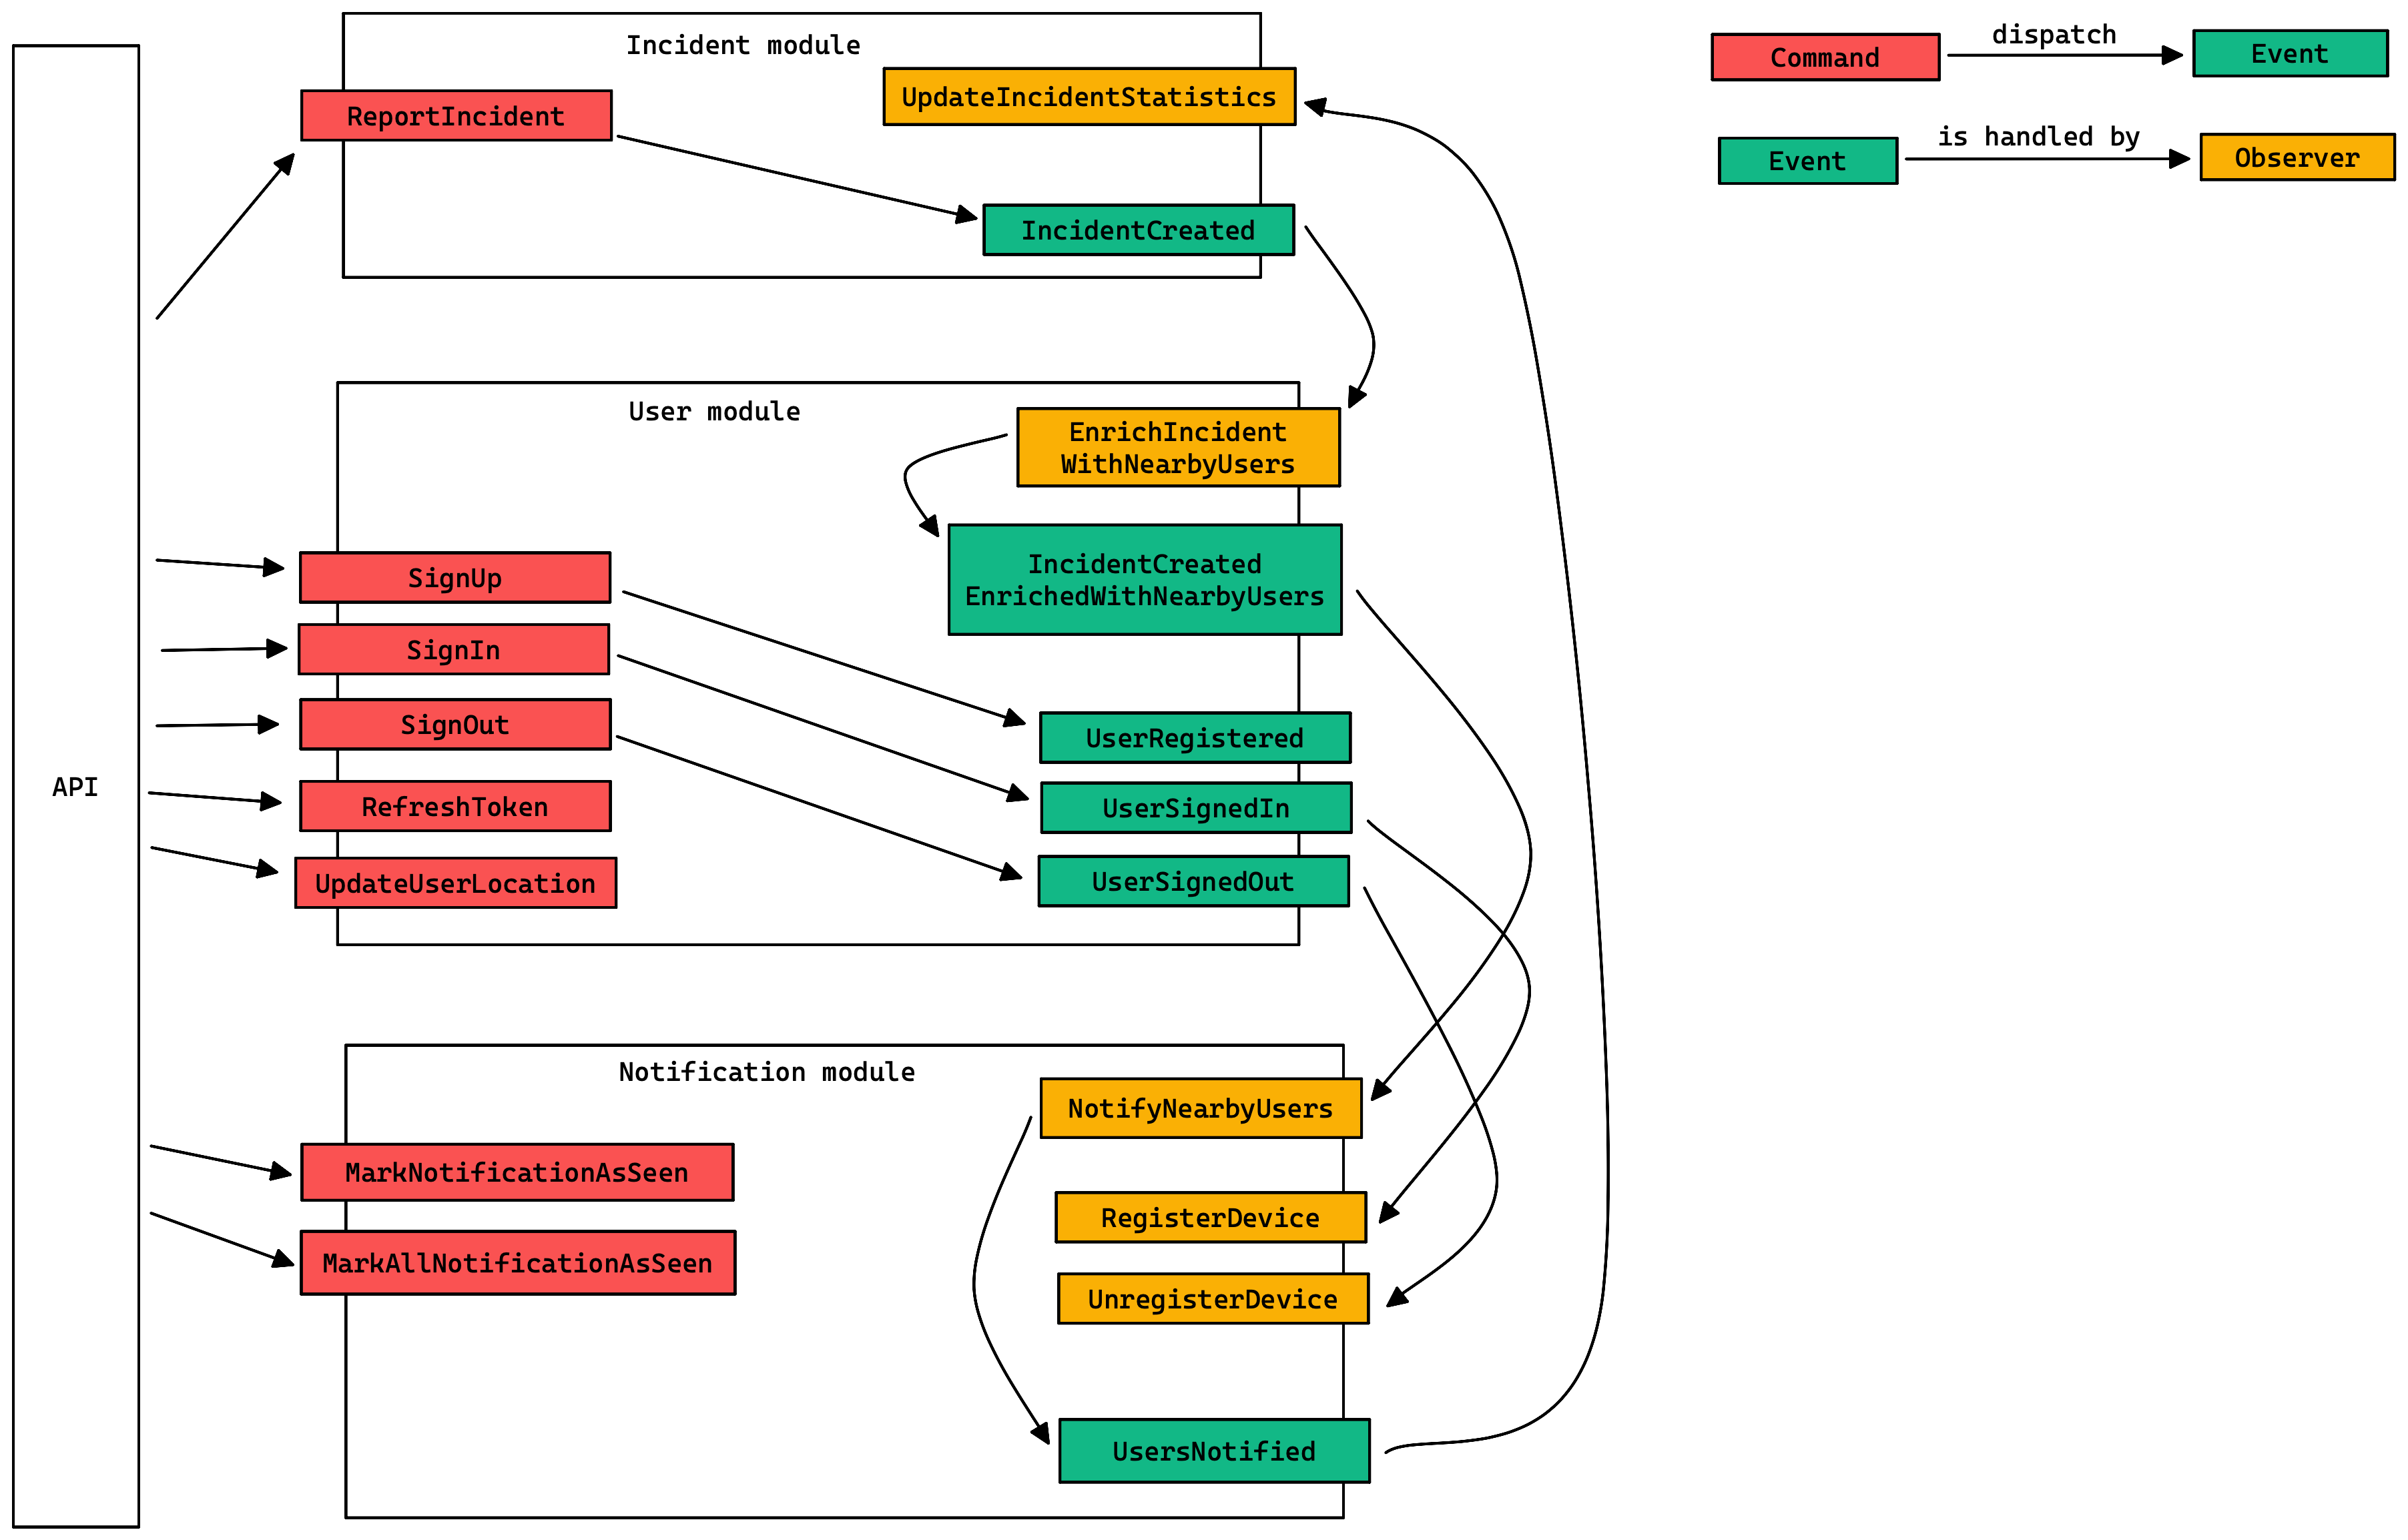
\includegraphics[width=\textwidth]{../diagrams/out/system_server_all_modules_commands-observers-events.png}
	\label{f.system_server_all_modules_commands-observers-events}
	\legend{\small Fonte: Elaborado pelo autor.}
\end{figure}

\FloatBarrier

\section{Comunicação entre servidor e aplicativo}

\subsection{GraphQL}
% vatangens do GraphQL: https://khalilstemmler.com/articles/graphql/graphql-architectural-advantages/#The-Data-Graph

GraphQL~\cite{graphql} é uma especificação e uma linguagem de consulta para APIs que permite com que clientes requisitem e recebam do servidor exatamente os dados que eles precisam. Ele possui seu próprio sistema de tipos e campos, ao contrário de \emph{endpoints} de um tradicional servidor HTTP que segue os princípios REST (\emph{Representational State Transfer}).

Para criar uma API GraphQL é necessário instalar uma biblioteca que o implementa na linguagem desejada, expor um \emph{endpoint} para receber as requisições GraphQL, definir um \texttt{GraphQL schema} e conectar os \texttt{resolvers} de cada campo aos seus respectivos \texttt{data sources}.

O \texttt{GraphQL schema} é definido em um arquivo declarativo e auto-documentável. Ele é conhecido tanto pelo servidor como pelo cliente e atua como uma camada virtual entre eles. Ele define um grafo com todos os dados que o servidor está expondo, assim como todas as operações disponíveis para a busca e alteração desses dados. Os dados que estão sendo expostos para consultas são definidos através de \texttt{GraphQL queries}, já os que estão sendo expostos para serem alterados, através de \texttt{GraphQL mutations}. Além deles, também existem as \texttt{GraphQL subscriptions}, usadas quando o cliente deseja ouvir por atualizações do servidor. Todos eles, juntos, são chamados de \texttt{GraphQL operations}.

\subsection{Do aplicativo ao módulo do servidor}

A Figura~\ref{f.system_server_api} ilustra de forma mais detalhada como o aplicativo se comunica com o servidor. Para \texttt{GraphQL queries} e \texttt{GraphQL mutations} há um fluxo síncrono de requisição-resposta onde é utilizado o protocolo HTTP, enquanto que para \texttt{GraphQL subscriptions} há um fluxo assíncrono e onde é estabelecida uma conexão persistente via o protocolo WebSocket para que o servidor possa também enviar atualizações ao cliente sem que haja uma requisição prévia feita por ele. Isso permite com que o usuário visualize os dados mais atualizados possíveis na tela. Alertas criados próximo à um usuário que está com o aplicativo aberto é um exemplo de atualização enviada apenas pelo servidor através de uma \texttt{GraphQL subscription}, a qual a aplicação cliente fica ``ouvindo'' desde o momento em que é iniciada.

\begin{figure}[htbp]
	\caption{\small Interação detalhada entre cliente e servidor.}
	\centering
	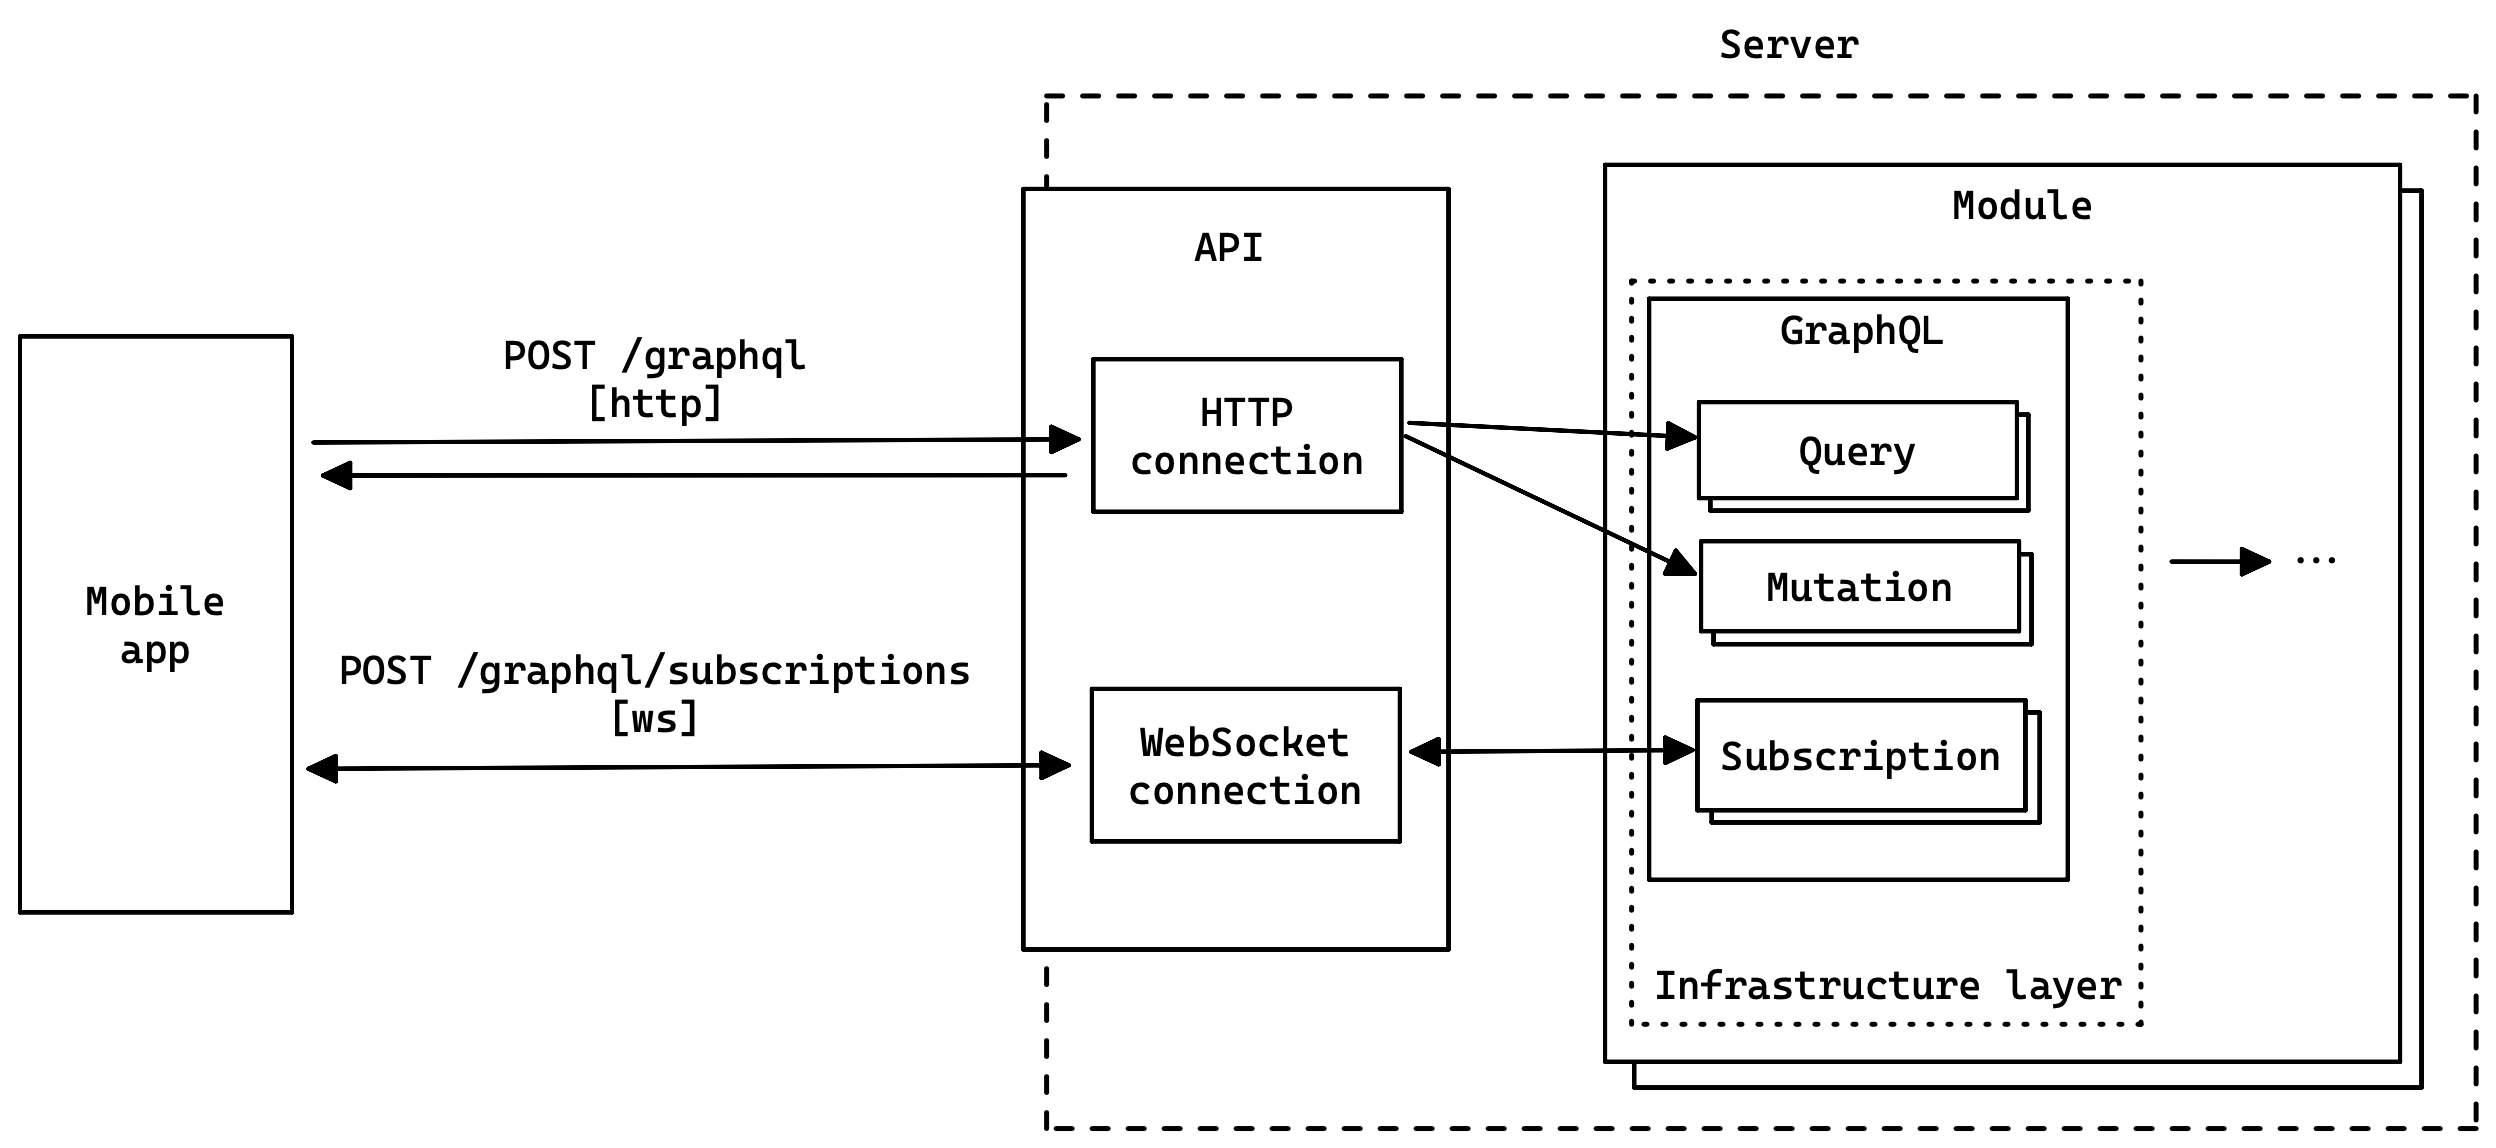
\includegraphics[width=\textwidth]{../diagrams/out/system_server_api.png}
	\label{f.system_server_api}
	\legend{\small Fonte: Elaborado pelo autor.}
\end{figure}

\FloatBarrier

\section{Aplicativo}

Para o funcionamento completo do aplicativo é exigido que o usuário forneça as seguintes permissões de acesso ao sistema operacional do dispositivo: compartilhamento da localização quando o aplicativo está em uso e também quando não está; uso da câmera e do microphone; e o envio de notificações. 

\subsection{Principais tecnologias}

Para a escrita do aplicativo foi utilizado o React Native~\cite{react-native}. O React Native é um framework Javascript para a construção de aplicações móveis multiplataforma, ou seja, que são renderizadas para o código nativo do iOS e do Android, e que é baseado no React~\cite{react}, uma biblioteca Javascript para a contrução de interfaces de usuário de forma declarativa.

Para melhorar a experiência de desenvolvimento com o React Native, foi utilizado o Expo~\cite{expo}, um \emph{React Native runtime} e SDK (\emph{Software Development Kit}). Entre as principais dependências, estão: Recoil~\cite{recoil}, uma biblioteca para gerenciamento de estado global no React; React Navigation~\cite{react-navigation}, uma biblioteca de navegação de telas no React Native; e Relay~\cite{relay}, descrito com mais detalhes na próxima seção.

\subsection{Busca e gerenciamento de dados com Relay}

O Relay~\cite{relay} é um framework para busca e gerenciamento de dados com GraphQL para React e React Native. Sem ele, consultas são facilmente duplicadas entre diferentes componentes, podem existir carregamentos em cascata de uma árvore de componentes (ou seja, cada componente filho começa a buscar os dados que precisa no servidor somente após o térmido da busca do seu componente pai), o que torna as consultas muito lentas e consequentemente prejudica a experiência do usuário. Em resumo, ao adotar Relay é possivel declarar quais dados cada componente precisa carregar antes de renderezar. O próprio framework se responsabiliza por buscar esses dados da forma mais perfomática e otimizada possível, evitando os problemas citados anteriormente.

A \texttt{Relay Store} é onde o Relay mantém todos os dados retornados pelas \texttt{GraphQL operations} que foram executadas. Cada dado possui um id único, e é através dele que é mantido um \emph{cache} para evitar buscas duplicadas de dados no servidor. Esses valores em \emph{cache} são atualizados pelo framework à cada nova resposta do servidor, mas também podem ser atualizados manualmente através dos \emph{optimistic updates}. Um \emph{optimistic update} permite evitar a espera da resposta do servidor para que algo seja refletido na tela do usuário. Por exemplo, se o usuário clicou em uma notificação, ela já pode ser renderizada como vista antes do servidor responder, pois provavelmente será uma requisição de sucesso.

Na Figura~\ref{f.system_app} todos os fluxos possíveis são ilustrados. As \texttt{actions} podem ser entendidas como qualquer ação realizada pelo usuário que solicite uma mudança de dados, como, por exemplo, clicar no botão para registrar um novo usuário ou adicionar um novo alerta. No caso, isso vale apenas para os componentes que declaram dependência de dados do servidor.

\begin{figure}[htbp]
	\caption{\small Busca de dados no aplicativo.}
	\centering
	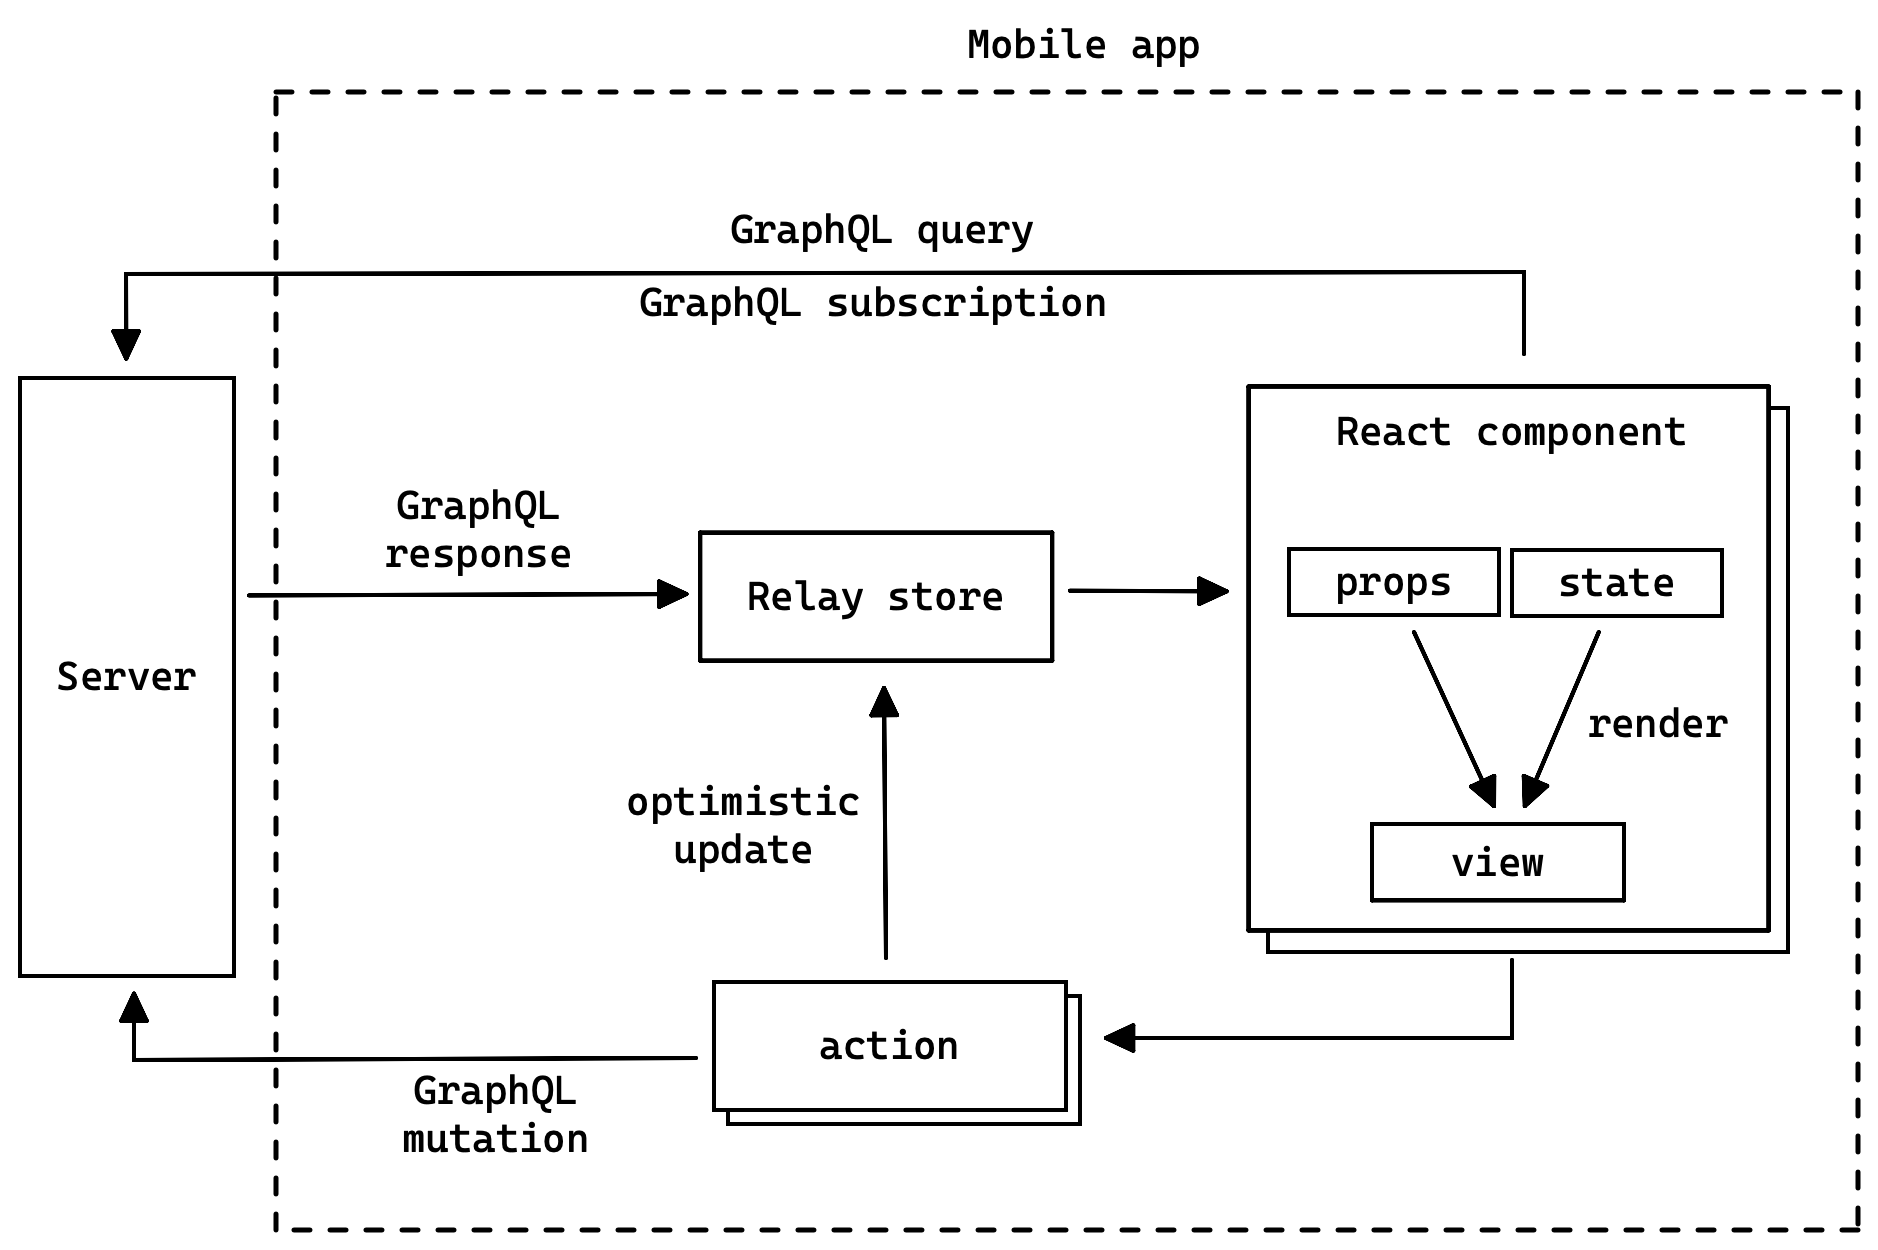
\includegraphics[width=\textwidth]{../diagrams/out/system_app.png}
	\label{f.system_app}
	\legend{\small Fonte: Elaborado pelo autor.}
\end{figure}

\FloatBarrier

\subsection{Inicialização do aplicativo}

A cada vez que o usuário realiza um novo \emph{login} mediante à inserção de usuário e senha corretos, um \emph{access token} é retornado pelo servidor, e ele, por sua vez, é criptografado e salvo no sistema de arquivos do dispositivo em formato de chave-valor. É lendo essa estrutura à cada inicialização do aplicativo, portanto, que é possível saber se o usuário já está logado ou não. O \emph{access token} gerado possui um prazo de expiração de 1 dia. No caso de ele estar expirado, ainda há um \emph{refresh token}, que é usado para gerar outro \emph{access token} válido de forma transparente ao usuário, e esse \emph{refresh token}, por sua vez, possui um prazo de expiração de 15 dias.

O aplicativo pode estar em dois estados. Ou ele está em \emph{foreground}, quando está aberto e ativo em primeiro plano, ou ele está em \emph{background}, quando está fechado ou em segundo plano. Como descrito pela Figura~\ref{f.system_app_initialization-flow}, após cada \emph{login} efetuado com sucesso algumas rotinas são executadas dependendo de qual for o estado do aplicativo. As rotinas 1 e 2 são executadas apenas no primeiro acesso ao aplicativo.

\begin{figure}[htbp]
	\caption{\small Fluxo de inicialização do aplicativo.}
	\centering
	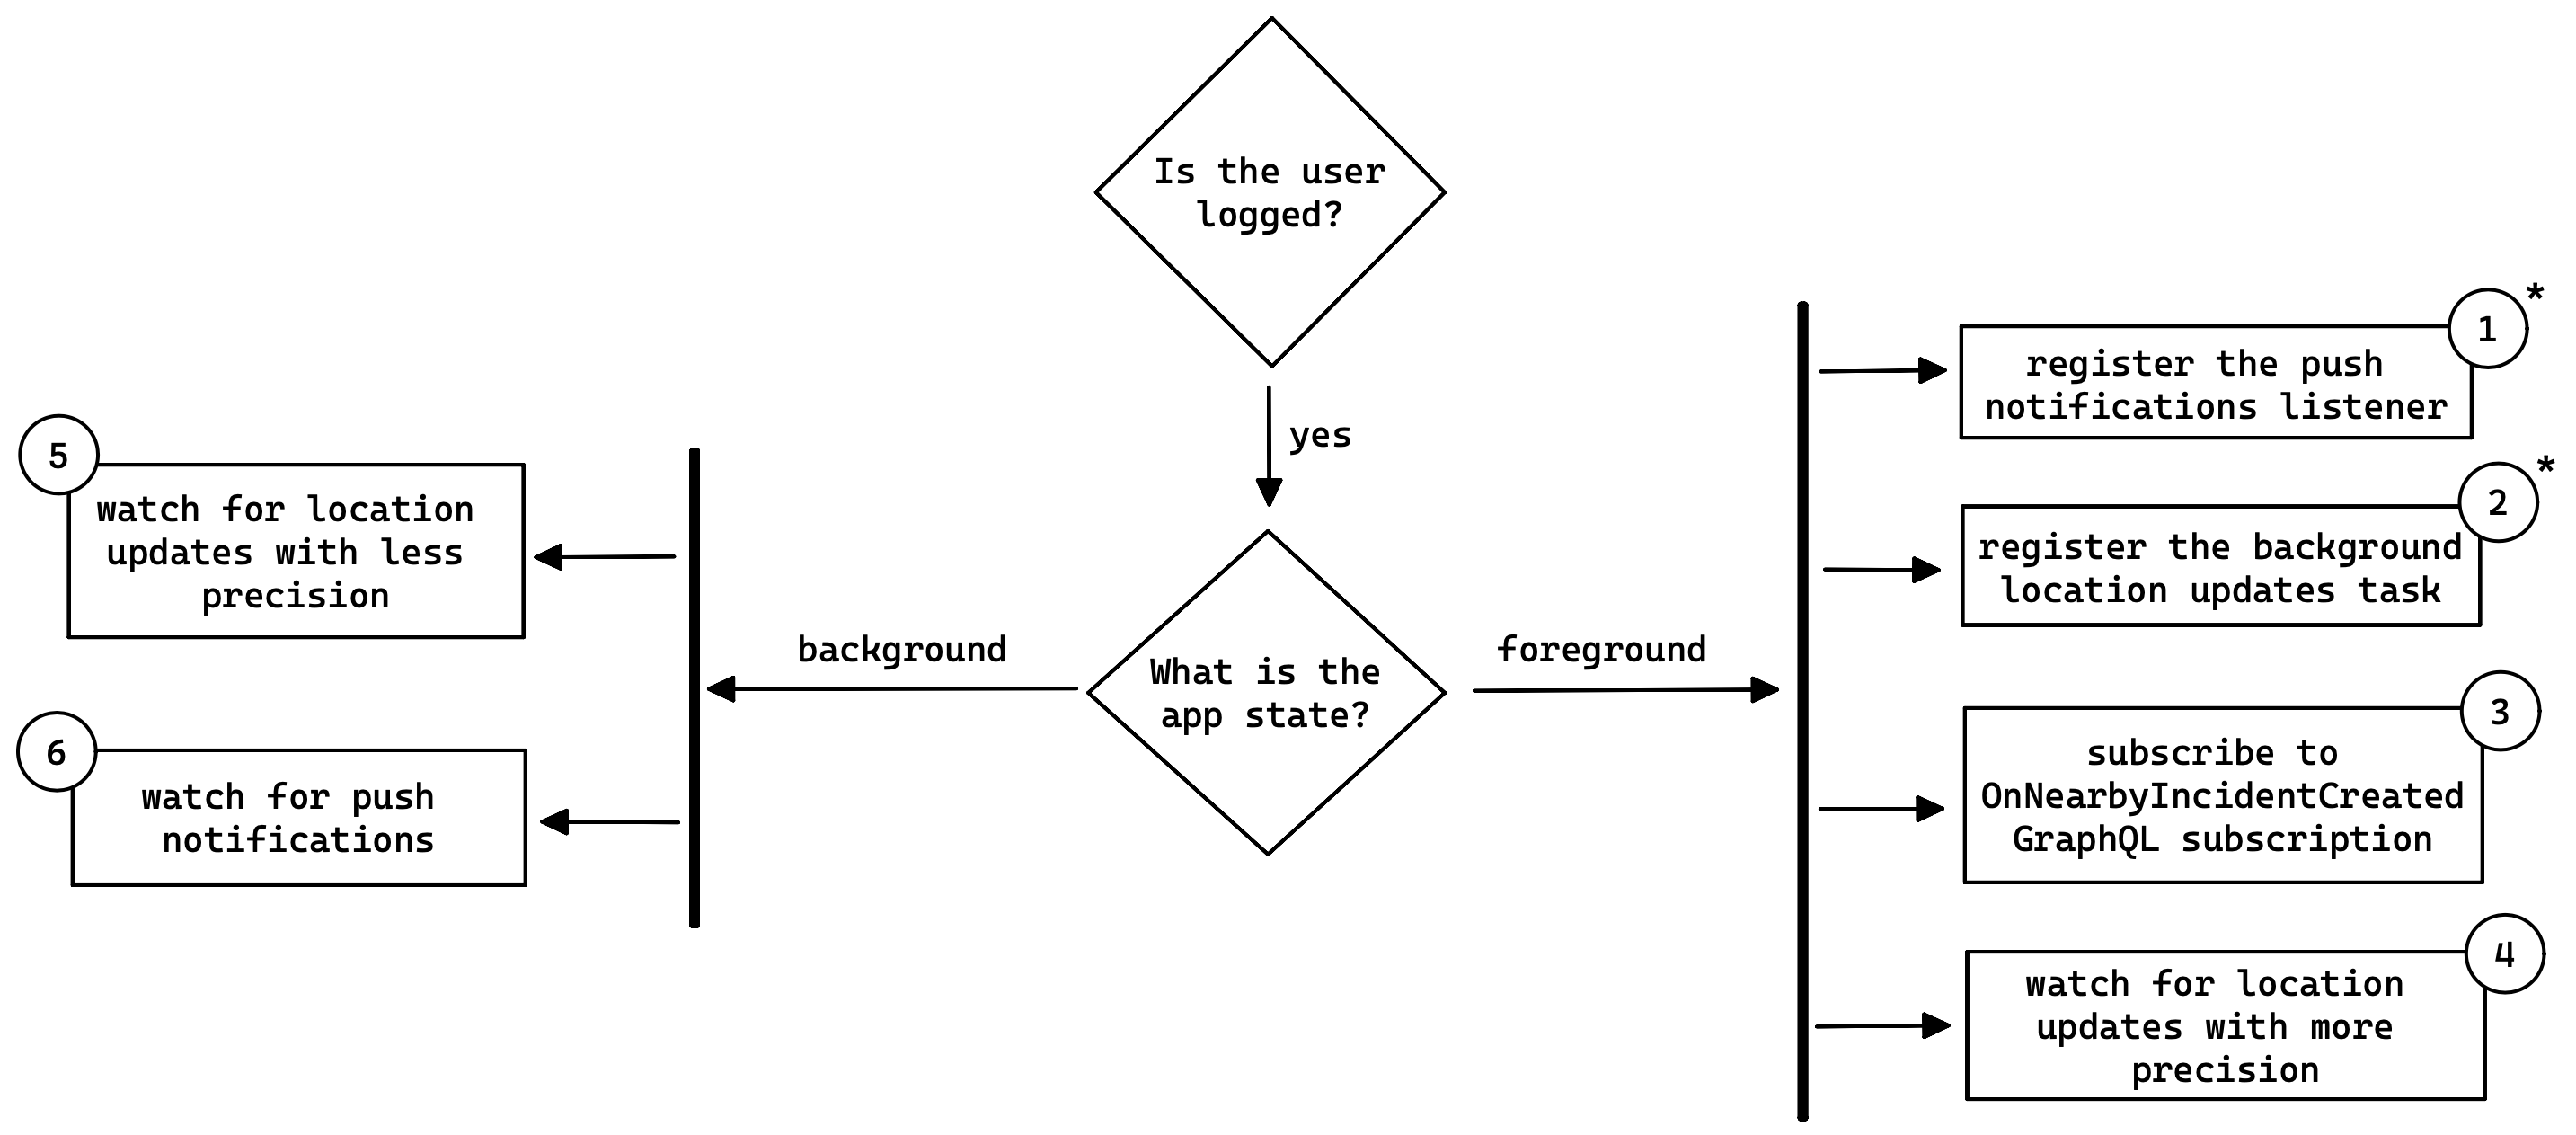
\includegraphics[width=\textwidth]{../diagrams/out/system_app_initialization-flow.png}
	\label{f.system_app_initialization-flow}
	\legend{\small Fonte: Elaborado pelo autor.}
\end{figure}

\FloatBarrier

Em relação às rotinas executadas em \emph{foreground}:

\begin{itemize}
	\item \textbf{1}: é definida a função que deve ser executada à cada vez que o usuário interage com uma \emph{push notification}, a qual redireciona o usuário para a tela relevante e marca a notificação como vista no servidor;
	\item \textbf{2}: é definida a \emph{background task} que será executada à cada nova atualização de localização do dispositivo. A implementação dessa \emph{background task} apenas atualiza o servidor com a nova localização;
	\item \textbf{3}: é feita a subscrição que receberá atualizações de cada novo alerta que for criado nas proximidades da localização atual do usuário, para que os novos alertas sejam renderizados em tempo real no mapa;
	\item \textbf{4}: ouve por atualizações de localização que ocorrem em pelo menos 100 milissegundos ou se a nova localização está com mais de 50 metros de distância em relação à última atualização. Para nova localização, o mapa é re-renderizado com a nova posição do usuário.
\end{itemize}

E em relação às rotinas executadas em \emph{background}:

\begin{itemize}
	\item \textbf{5}: a \emph{background task} definida no primeiro acesso é executada baseada em duas condições. Ou à cada 10 segundos ou se houve uma mudança de localização com uma distância de mais de 100 metros em relação à última localização;
	\item \textbf{6}: ouve por novas \emph{push notifications} que eventualmente chegam no dispositivo.
\end{itemize}

\subsection{Telas}

A Figura~\ref{f.lazarus-sign} mostra, à direita, o formulário de registro de um novo usuário e, à esquerda, o formulário de \emph{login}.

\begin{figure}[htbp]
	\caption{\small Telas de \emph{login} e de registro de usuário} 
	\begin{center}
		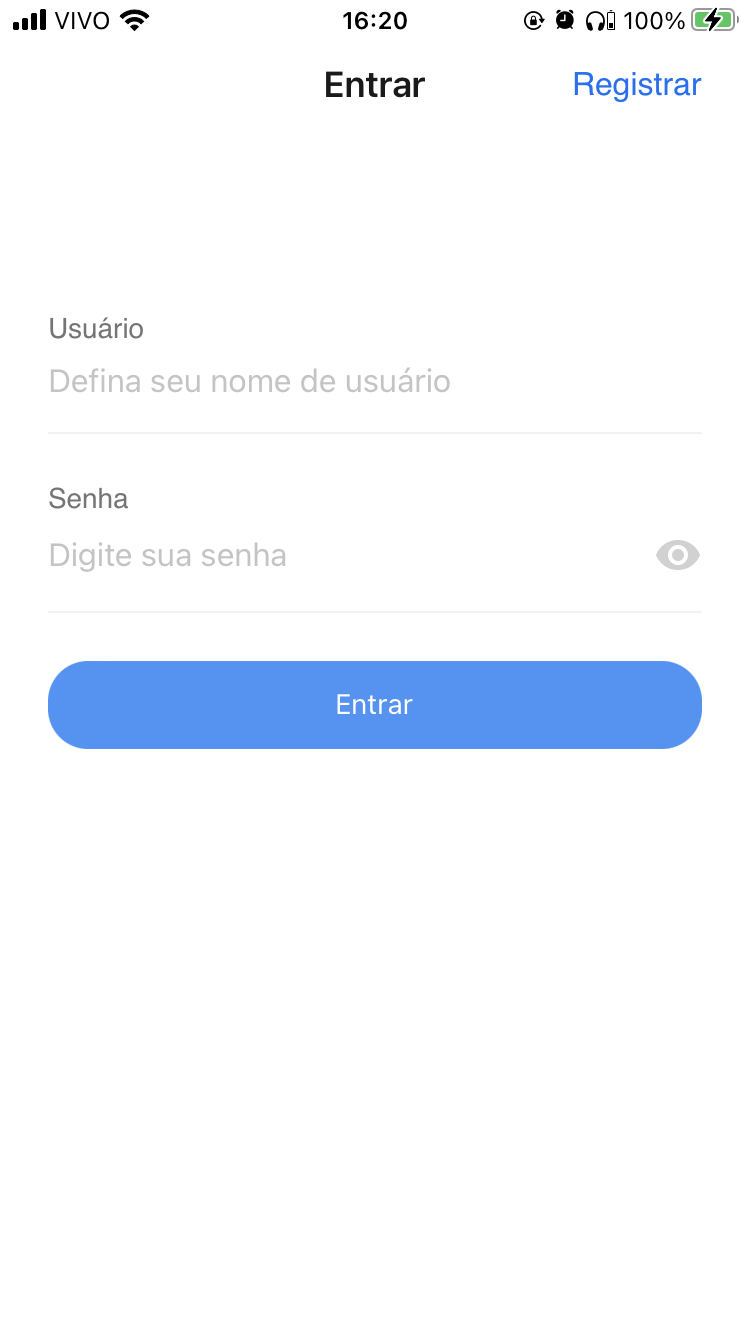
\includegraphics[height=8cm]{images/lazarus-sign-in.png} \quad
		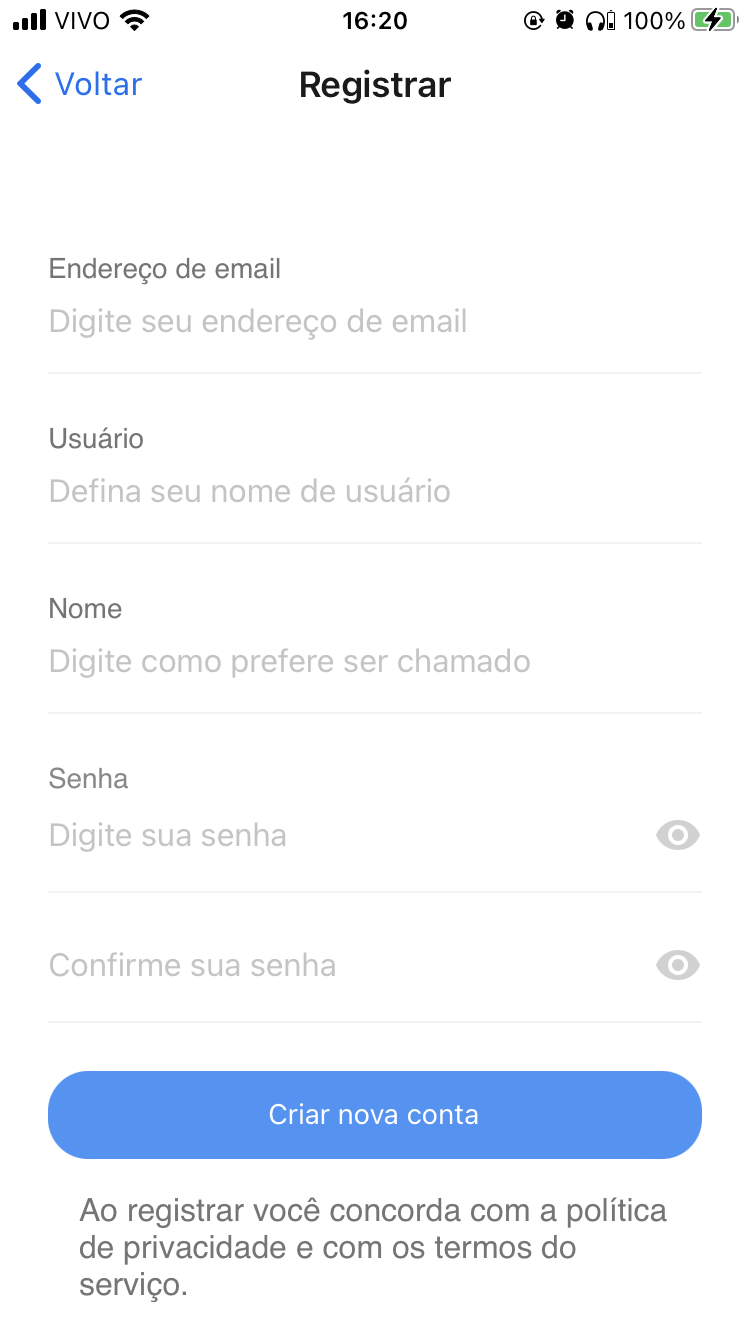
\includegraphics[height=8cm]{images/lazarus-sign-up.png}
	\end{center}
	\label{f.lazarus-sign}
	\legend{\small Fonte: Elaborado pelo autor.}
\end{figure}

\FloatBarrier

A Figura~\ref{f.lazarus-explorer} mostra, à esquerda, a primeira tela que um usuário encontra após ter realizado o \emph{login} com sucesso, onde é possível visualizar um mapa com todos os alertas mais próximos à localicação atual do usuário, e também navegar para as demais telas através da barra de navegação inferior. À direita, é mostrado como a tela varia quando um alerta é selecionado no mapa.

\begin{figure}[htbp]
	\caption{\small Tela inicial} 
	\begin{center}
		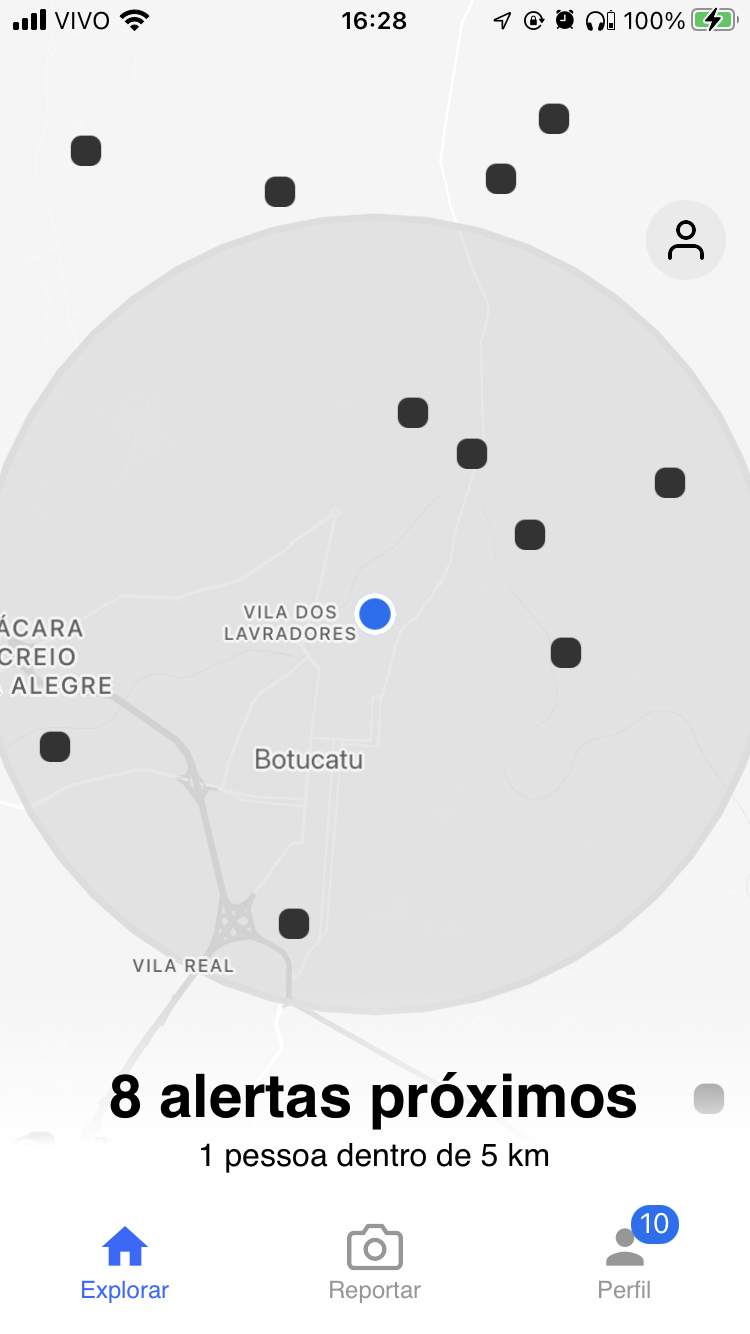
\includegraphics[height=8cm]{images/lazarus-explorer-1.png} \quad
		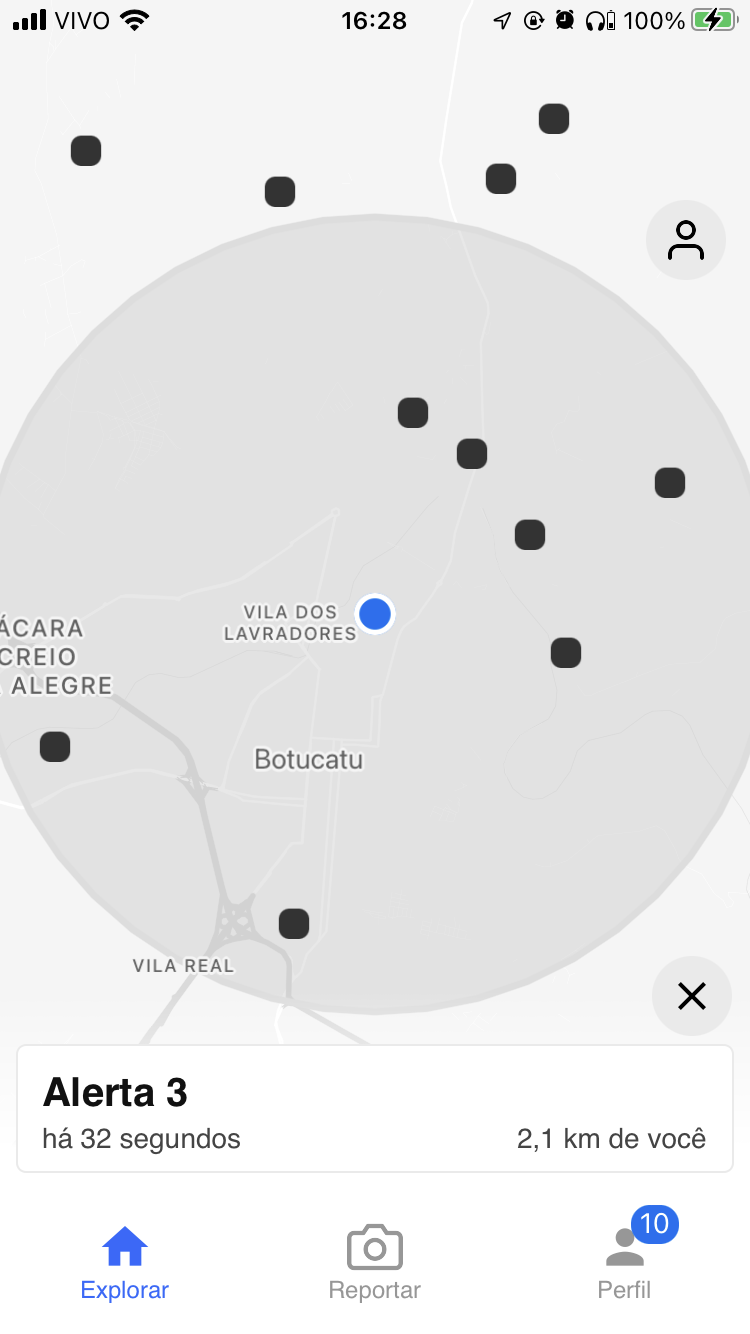
\includegraphics[height=8cm]{images/lazarus-explorer-2.png}
	\end{center}
	\label{f.lazarus-explorer}
	\legend{\small Fonte: Elaborado pelo autor.}
\end{figure}

\FloatBarrier

A Figura~\ref{f.lazarus-incident} mostra a tela de um único alerta expandido, onde é possível ver suas imagens e vídeos, qual usuário que o reportou e informações relativas ao usuário ``logado''.

\begin{figure}[htbp]
	\caption{\small Tela de um alerta} 
	\centering
	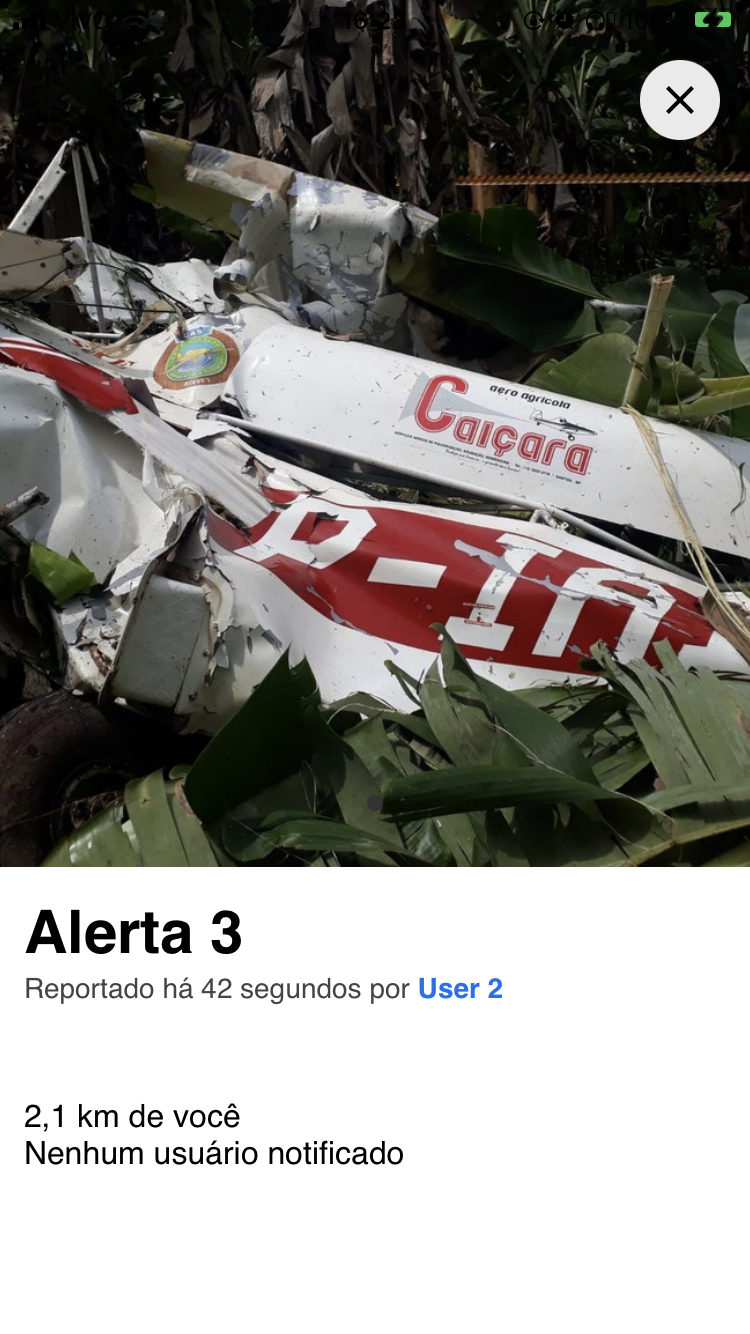
\includegraphics[height=8cm]{images/lazarus-incident.png}
	\label{f.lazarus-incident}
	\legend{\small Fonte: Elaborado pelo autor.}
\end{figure}

\FloatBarrier

A Figura~\ref{f.lazarus-profile}, à esquerda, mostra a tela de perfil, que contém informações específicas do usuário ``logado'' e dá acesso à tela de notificações e de preferências. À direita, é mostrado a tela de notificações, onde o usuário pode checar se perdeu alguma notificação, navegar para o alerta mencionado ao clicar na notificação, e marcar uma notificação como lida.

\begin{figure}[htbp]
	\caption{\small Telas do perfil do usuário e de notificações} 
	\begin{center}
		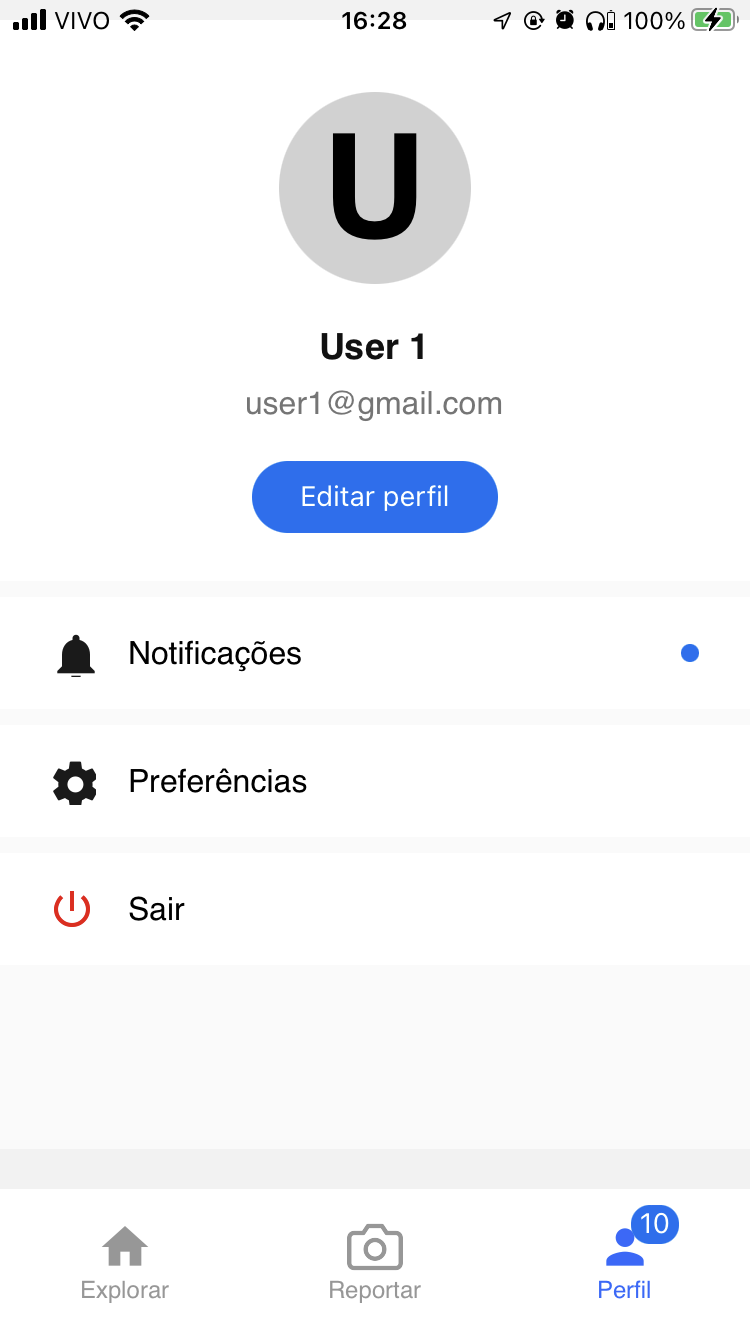
\includegraphics[height=8cm]{images/lazarus-profile.png}
		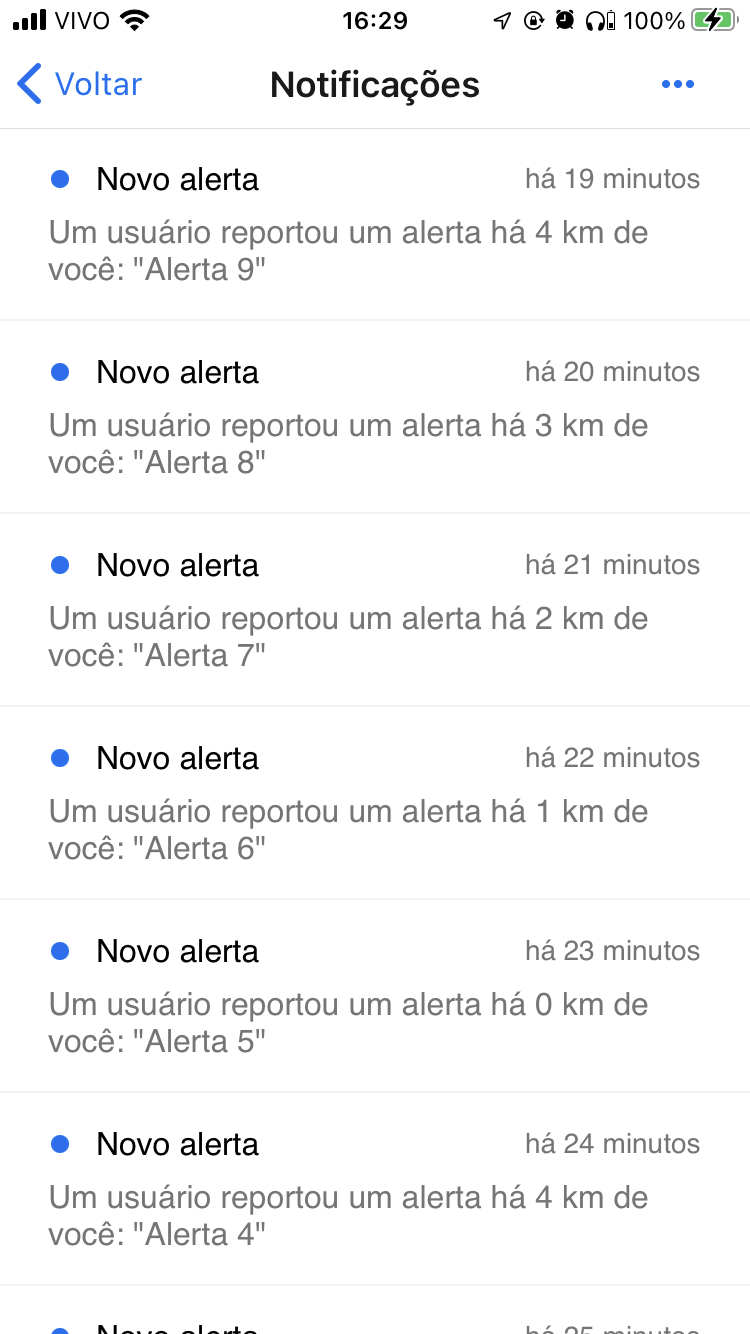
\includegraphics[height=8cm]{images/lazarus-notifications.png}
	\end{center}
	\label{f.lazarus-profile}
	\legend{\small Fonte: Elaborado pelo autor.}
\end{figure}

\FloatBarrier

A Figura~\ref{f.lazarus-reporting} mostra todas as telas que fazem parte do fluxo de publicação de um novo alerta. Da esquerda para direita, temos a câmera, a tela de revisão das imagens e vídeos, e o formulário para inserção do título do alerta que está sendo publicado.

\begin{figure}[htbp]
	\caption{\small Telas de publicação de um alerta} 
	\begin{center}
		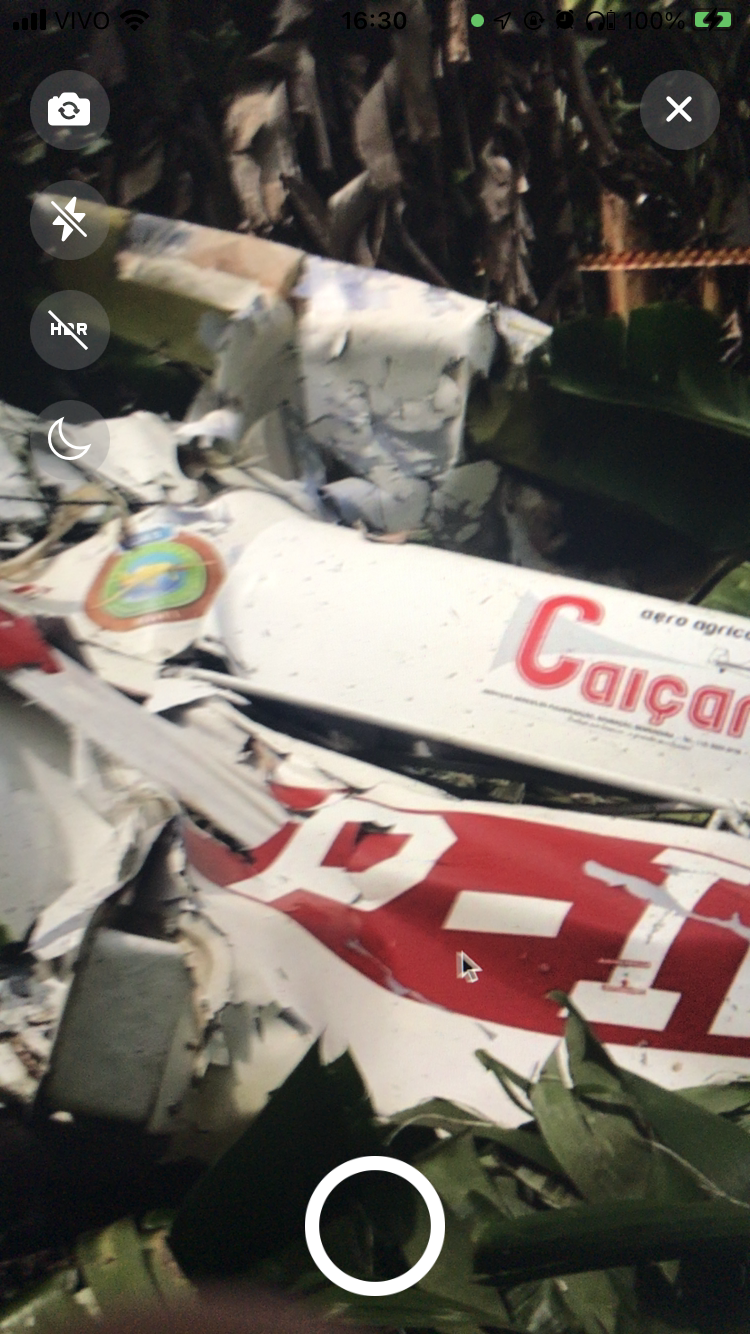
\includegraphics[height=8cm]{images/lazarus-camera.png}
		
\includegraphics[height=8cm]{images/lazarus-reporting-1.png} \quad
		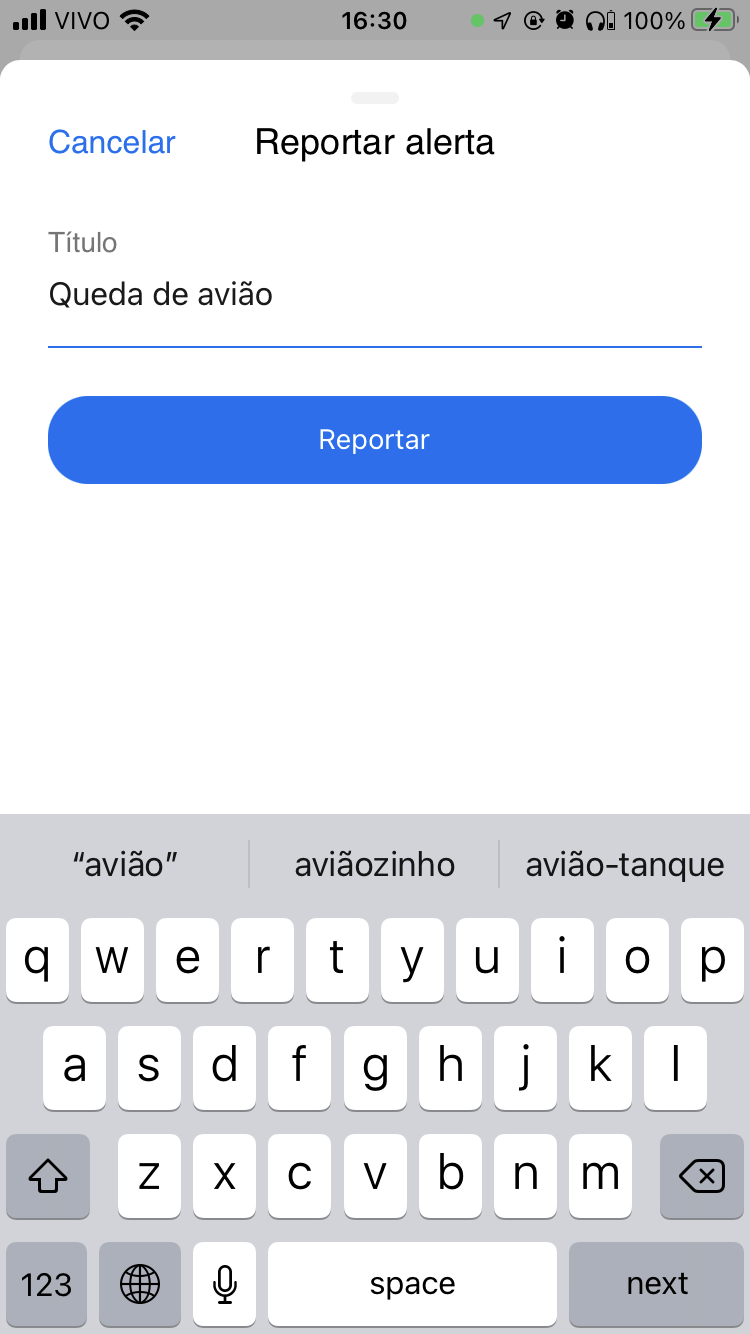
\includegraphics[height=8cm]{images/lazarus-reporting-2.png}
	\end{center}
	\label{f.lazarus-reporting}
	\legend{\small Fonte: Elaborado pelo autor.}
\end{figure}

\FloatBarrier

\section{Outras tecnologias}

Além das tecnologias já citadas, outras tecnologias que não estão relacionadas apenas ao servidor ou ao aplicativo também foram utilizadas.

\begin{itemize}
	\item Typescript~\cite{typescript}: sistema de tipos para Javascript. Utilizado tanto  no aplicativo quanto no servidor;
	\item Terraform~\cite{terraform}: ferramenta de IaC (\emph{Infrastructure as Code}) para gerenciamento serviços em nuvem via arquivos de configuração declarativos;
	\item Docker~\cite{docker}: ferramenta de virtualização à nível do sistema operacional baseado em containers isolados. Utilizado durante o desenvolvimento.
\end{itemize}
